\documentclass[11pt]{article}

% ---------------------------------------------------------------------------
% Equilibrium Bifurcations and Periodic Dynamics in a Planar Restricted
% Five-Body Problem with Four Unequal Primaries
%
% Tables in tables/ and figures in figures/ are AUTO-GENERATED from the
% verified result CSVs (paper/make_tables.py, scripts/make_*_figures.py).
% Full coordinates, result CSVs, scripts, and tests are in the accompanying
% code/data reproducibility repository (see the Data and code availability section).
% ---------------------------------------------------------------------------

\usepackage[margin=1in]{geometry}
\usepackage{amsmath,amssymb,amsthm}
\usepackage{graphicx}
\usepackage{booktabs}
\usepackage[hidelinks]{hyperref}
\usepackage{microtype}
\setlength{\emergencystretch}{3em}

\graphicspath{{figures/}}

\newtheorem{theorem}{Theorem}
\newtheorem{lemma}{Lemma}
\newtheorem{remark}{Remark}

% consistent notation
\newcommand{\Om}{\Omega}
\newcommand{\Ox}{\Omega_x}
\newcommand{\Oy}{\Omega_y}
\newcommand{\Oxx}{\Omega_{xx}}
\newcommand{\Oxy}{\Omega_{xy}}
\newcommand{\Oyy}{\Omega_{yy}}
\newcommand{\rzero}{\rho_0}
\newcommand{\rone}{\rho_1}
\newcommand{\rtwo}{\rho_2}
\newcommand{\CJ}{C_J}
\newcommand{\grad}{\nabla}
\newcommand{\R}{\mathbb{R}}

\title{Equilibrium Bifurcations and Periodic Dynamics in a Planar
Restricted Five-Body Problem with Four Unequal Primaries}

% AUTHORS: replace the \thanks placeholders with the real affiliations before submission
\author{Muhammad Shoaib\thanks{Affiliation to be finalized.} \and
        A.~R.~Kashif\thanks{Affiliation to be finalized.}}
\date{\today}

\begin{document}
\maketitle


\begin{abstract}
We investigate the planar restricted five-body problem in which four
unequal primaries form a non-symmetric coplanar central configuration and
an infinitesimal fifth body moves in the associated uniformly rotating
field. After implementing and validating the model, we fix
$(a,b)=(0.9,-0.1)$ and continue the admissible central configurations in
the remaining geometric parameters. The principal result is structural:
on this slice the admissible set $\psi=0$ separates numerically into two
distinct connected components, so configurations with different
equilibrium multiplicities need not belong to a single continuous family.
Pseudo-arclength continuation combined with independent multi-start
equilibrium searches reveals the interior cascades
\[
5\rightarrow7\rightarrow5
\qquad\text{and}\qquad
7\rightarrow9\rightarrow11\rightarrow9\rightarrow7\rightarrow5.
\]
All seven interior count changes are generic saddle-node folds, verified
through an augmented degeneracy system, nondegeneracy conditions, and the
local scaling
\[
d\propto|\ell-\ell_c|^{1/2}.
\]
The eleven-equilibrium regime exhibits a branch exchange: the pair created
at the $9\rightarrow11$ fold is distinct from the pre-existing pair
destroyed at the subsequent $11\rightarrow9$ fold. Both admissible
components contain reliably resolved intervals of spectrally stable
equilibria. From selected simple centre modes we continue ten Lyapunov
periodic-orbit families comprising 198 corrected periodic solutions with
closure residuals below $10^{-10}$. Families continued from the selected
doubly-elliptic parents remain Floquet stable over the computed intervals,
whereas those continued from selected saddle$\times$centre parents are
real unstable. Selected near-commensurate families approach the
period-doubling threshold; the closest, on family~10, reaches
$|\nu+2|\simeq10^{-7}$ but turns back without crossing. Finally, critical
Jacobi levels are used to demonstrate a resolution-robust representative
change in Hill-region connectivity and to place selected periodic families
within their accessible regions. All conclusions concerning
central-configuration connectivity and equilibrium multiplicity are
numerical and specific to the investigated parameter slice.
\end{abstract}

\section{Introduction}
\label{sec:intro}

Restricted $n$-body models, in which an infinitesimal body moves in the gravitational field of a prescribed relative equilibrium of massive primaries, provide a classical setting for studying the organization of celestial-mechanical phase space. In the circular restricted three-body problem (CR3BP), the five Lagrange equilibria, their linear stability, the associated zero-velocity curves and Hill regions, and the periodic-orbit families emanating from them are well understood \cite{szebehely1967,meyerhalloffin2009}. Higher restricted problems retain this basic structure but introduce an additional dependence on the geometry and mass distribution of the primaries: both the number of relative equilibria and their dynamical character can change as the primary configuration is varied.

This dependence is already apparent in the restricted four-body problem. For three primaries in the Lagrange equilateral configuration, the locations, number, and stability of the libration points vary with the primary mass ratios, and the problem supports extensive families of periodic orbits \cite{baltagiannispapadakis2011a,baltagiannispapadakis2011b}; the stability of the corresponding four-body relative equilibria was analysed earlier by Sim\'o \cite{simo1978}. Baltagiannis and Papadakis also extended the periodic-orbit analysis to configurations with three unequal primaries, including the linear stability of the resulting families \cite{baltagiannispapadakis2011b}. In contrast, we are not aware of an analogous periodic-orbit study in the restricted five-body problem in which all four primaries have distinct masses and form a general non-symmetric central configuration.

Restricted five-body models introduce a further level of geometric freedom. Ollongren considered four primaries in a symmetric configuration and obtained nine libration points, including stable equilibria \cite{ollongren1988}. Subsequent studies have examined regular-polygon and other symmetric arrangements \cite{kalvouridis1999}, numerical basins of attraction of the equilibria \cite{zotossuraj2018}, and networks of symmetric and non-symmetric periodic orbits \cite{zotospapadakis2019}. These investigations demonstrate that the restricted five-body problem can possess a substantially richer equilibrium and periodic-orbit structure than the CR3BP.

A crucial additional constraint is that the primaries cannot, in general, be placed arbitrarily. To remain fixed relative to one another in a uniformly rotating frame, they must themselves form a central configuration (CC). The geometry and multiplicity of four-body central configurations have therefore long been studied independently of the restricted problem, from the classical work of Moulton \cite{moulton1900} to later results on their stability, bifurcation structure, and finiteness \cite{simo1978,hamptonmoeckel2006}. Many tractable four-body families impose some form of symmetry, such as equal masses, reflection symmetry, or a kite or trapezoidal geometry \cite{stevesroy1998,benhammouda2020}. Such assumptions reduce the dimensionality of the CC problem and can permit partly analytic treatment, but they also restrict the set of primary geometries accessible to the infinitesimal body.

The general coplanar four-body formulation of Shoaib et al.\ \cite{shoaib2023} removes this restriction. After normalization, three primaries define a reference triangle while the fourth is free in the plane; the four masses are then determined, up to scale, by a scalar central-configuration constraint together with positivity conditions on the resulting mass ratios. The admissible primary configurations therefore form a nontrivial subset of a continuous geometric parameter space rather than a prescribed symmetric family. Introducing an infinitesimal fifth body into this rotating four-primary configuration leads naturally to the question considered here:

\begin{quote}
\emph{How do the equilibrium structure and the associated local nonlinear dynamics of the restricted body change as the underlying non-symmetric four-primary central configuration is continuously deformed?}
\end{quote}

This question cannot be answered by comparing isolated parameter choices alone. Two configurations may possess different numbers of equilibria without belonging to the same connected component of the admissible CC set, in which case there is no bifurcation sequence directly connecting their equilibrium counts. Conversely, an individual admissible component may pass through equilibrium multiplicities not represented by the original sampled configurations. The topology of the primary CC set must therefore be determined together with the restricted equilibria if one wishes to understand how those equilibria are created, destroyed, and reorganized.

To our knowledge, existing studies of unequal or non-symmetric restricted four- and five-body problems predominantly analyse specified primary configurations or restricted parameter families rather than tracing the equilibrium structure along a continuously varying general four-body CC. Detailed continuation and periodic-orbit studies of restricted five-body models have, in particular, largely exploited prescribed symmetric primary configurations \cite{ollongren1988,kalvouridis1999,zotospapadakis2019}. We are not aware of a study that simultaneously follows an admissible non-symmetric four-primary CC family, determines the restricted equilibria along it, locates and classifies their bifurcations, tracks their linear stability, and then continues the periodic dynamics associated with the resulting centre modes. This is the gap addressed in the present work.

Our analysis combines pseudo-arclength continuation of the primary CC constraint with an independent global search for the equilibria of the infinitesimal body at each continuation point. The distinction is important: an equilibrium branch created at a saddle-node does not exist before the bifurcation and may therefore be missed if one merely continues previously known roots. Changes in the equilibrium count are bracketed and the corresponding critical configurations are refined by solving the equilibrium equations together with the Hessian-degeneracy condition. Genericity is tested through the fold transversality and quadratic-nondegeneracy conditions and independently through the local square-root scaling of the merging pair. Linear spectra are then followed along the resulting equilibrium branches. Centre modes at selected equilibria provide initial seeds for differential correction and continuation of nonlinear periodic-orbit families, whose stability is determined from their Floquet multipliers. Finally, the critical Jacobi values provide a geometric link between the equilibrium structure and the accessible Hill regions.
The principal results are as follows.


\begin{enumerate}

\item On the common Case-1/Case-2 slice
\[
(a,b)=(0.9,-0.1),
\]
the admissible four-primary CC set separates numerically into two distinct
connected components. Consequently, the five- and nine-equilibrium reference
configurations do not lie on a single fixed-$(a,b)$ continuation family.

\item Equilibrium multiplicity changes along the two admissible components
through seven generic saddle-node folds. The corresponding sequences are
\[
5\rightarrow7\rightarrow5
\]
on the first component and
\[
7\rightarrow9\rightarrow11\rightarrow9\rightarrow7\rightarrow5
\]
on the second. The eleven-equilibrium regime contains a nontrivial branch
exchange: the pair created at the $9\rightarrow11$ fold is distinct from the
pre-existing pair destroyed at the subsequent $11\rightarrow9$ fold.

\item Both admissible components contain intervals of spectrally stable
equilibria. Continuation from selected centre modes yields ten Lyapunov
periodic-orbit families. The families associated with the selected
doubly-elliptic parent equilibria remain Floquet stable over the computed
intervals, whereas those associated with selected saddle$\times$centre parents
are real unstable. Families seeded near low-order centre-frequency
commensurabilities approach the period-doubling threshold but do not cross it
within the computed continuation range.

\item The critical Jacobi values associated with the equilibrium branches
provide a direct connection between the bifurcation structure and the
geometry of the accessible region. A representative Hill-region connectivity
change is resolved numerically and related to the computed periodic motion.

\end{enumerate}
The principal conclusion is therefore not simply that the present asymmetric problem supports as many as eleven equilibria. Rather, on the investigated parameter slice, the \emph{topology of the admissible primary central-configuration set organizes which restricted equilibrium branches coexist and which bifurcation sequences are accessible}. The eleven-equilibrium state, the stable equilibrium intervals, and the associated periodic-orbit families arise as dynamical consequences of this organization. All statements concerning component connectivity and equilibrium completeness are numerical and apply to the chosen slice of the full four-parameter admissible set; continuation through the complete CC parameter space remains an open problem. 
\section{Mathematical model}
\label{sec:model}

We describe the model in normalized form. The four-body central-configuration
formulation of Section~\ref{subsec:cc} is due to \cite{shoaib2023}
and is \emph{not} claimed as a result of the present paper; we restate it only
to fix notation and because it defines the parameter family along which the
restricted problem is posed. The restricted fifth-body model follows in
Sections~\ref{subsec:potential}--\ref{subsec:jacobi}.

\subsection{The primary central configuration}
\label{subsec:cc}

Following the normalization of Shoaib et al.\ \cite{shoaib2023}, we use the
translation, rotation, reflection, and scaling invariances of the planar
central-configuration problem to place the four primaries at
\begin{equation}
\mathbf r_0=(0,b),\qquad
\mathbf r_1=(-1,0),\qquad
\mathbf r_2=(0,a),\qquad
\mathbf r_3=(c_1,c_2),
\label{eq:primary_positions}
\end{equation}
with
\[
a>0,\qquad b<a,\qquad b\neq \pm a.
\]
The choice $\mathbf r_1=(-1,0)$ fixes the length scale, while
$\mathbf r_0$ and $\mathbf r_2$ lie on the $y$-axis and
$\mathbf r_3=(c_1,c_2)$ remains free in the plane. The geometry is therefore
described by the parameter vector
\[
\mathbf p=(a,b,c_1,c_2).
\]

For compactness, define
\begin{equation}
\begin{aligned}
\sigma &= (1+a^2)^{3/2},
&
\varsigma &= (1+b^2)^{3/2},
&
\tau &= (a-b)^3,
\\
G &= \left[c_1^2+(c_2-a)^2\right]^{3/2},
&
T &= \left[c_1^2+(c_2-b)^2\right]^{3/2},
&
M &= \left[(c_1+1)^2+c_2^2\right]^{3/2}.
\end{aligned}
\label{eq:auxiliary_distances}
\end{equation}
These quantities are the cubes of the six mutual distances between the
primaries.

Let
\[
\rho_0=\frac{m_0}{m_3},\qquad
\rho_1=\frac{m_1}{m_3},\qquad
\rho_2=\frac{m_2}{m_3}
\]
denote the primary mass ratios. For the nondegenerate geometries considered
here, the coplanar four-body central-configuration condition of
\cite{shoaib2023} reduces to the scalar equation
\begin{equation}
\begin{aligned}
\psi(a,b,c_1,c_2)
={}&
\tau(\sigma-\varsigma)M
+T\left[(\tau-\sigma)M+\sigma(\varsigma-\tau)\right]
\\
&+
G\left[(\sigma-\varsigma)T+(\varsigma-\tau)M
+\varsigma(\tau-\sigma)\right]
=0,
\end{aligned}
\label{eq:cc_constraint}
\end{equation}
and the corresponding mass ratios are
\begin{equation}
\rho_0=
\frac{(c_2-a-ac_1)(M-G)\varsigma\tau}
     {(a-b)(\varsigma-\tau)MG},
\qquad
\rho_1=
\frac{c_1(G-T)\sigma\varsigma}
     {(\sigma-\varsigma)GT},
\qquad
\rho_2=
\frac{(c_2-b-bc_1)(M-T)\sigma\tau}
     {(a-b)(\tau-\sigma)MT}.
\label{eq:mass_ratios}
\end{equation}
Equations~\eqref{eq:cc_constraint}--\eqref{eq:mass_ratios} are the
four-body central-configuration result of \cite{shoaib2023}; they are
restated here only to define the family of primary configurations used in
the restricted problem.

Not every solution of $\psi=0$ corresponds to a positive-mass,
nondegenerate configuration. We therefore define the admissible set
\begin{equation}
\mathcal A=
\left\{
\mathbf p:
\psi(\mathbf p)=0,\;
\rho_0(\mathbf p)>0,\;
\rho_1(\mathbf p)>0,\;
\rho_2(\mathbf p)>0
\right\},
\label{eq:admissible_set}
\end{equation}
subject additionally to non-vanishing denominators in
\eqref{eq:mass_ratios} and the exclusion of primary collisions. Since only
mass ratios enter the central-configuration construction, the overall mass
scale remains arbitrary. We fix this scale by setting $m_3=1$, so that the
normalized primary masses used throughout the restricted problem are
\[
(m_0,m_1,m_2,m_3)=(\rho_0,\rho_1,\rho_2,1).
\]

\subsection{The restricted fifth body: potential, equilibria, and linear stability}
\label{subsec:potential}

For each admissible primary configuration
$\mathbf p\in\mathcal A$, the four primary masses and positions are fixed in
the uniformly rotating frame, and the fifth body is taken to be
infinitesimal: it moves in their gravitational field but does not perturb
the primary central configuration. Let $(x,y)$ denote its rotating-frame
coordinates, and define the distances to the four primaries by
\begin{equation}
\begin{aligned}
r_{40} &= \sqrt{x^2+(y-b)^2},
&
r_{41} &= \sqrt{(x+1)^2+y^2},
\\
r_{42} &= \sqrt{x^2+(y-a)^2},
&
r_{43} &= \sqrt{(x-c_1)^2+(y-c_2)^2}.
\end{aligned}
\label{eq:test_particle_distances}
\end{equation}

With the rotation rate normalized to unity, the effective potential is
\begin{equation}
\Omega(x,y)
=
\frac{1}{2}(x^2+y^2)
+
\sum_{i=0}^{3}\frac{m_i}{r_{4i}},
\label{eq:effective_potential}
\end{equation}
where
\[
(m_0,m_1,m_2,m_3)
=
(\rho_0,\rho_1,\rho_2,1).
\]
The equations of motion are
\begin{equation}
\ddot{x}-2\dot{y}=\Omega_x,
\qquad
\ddot{y}+2\dot{x}=\Omega_y,
\label{eq:equations_of_motion}
\end{equation}
with
\begin{equation}
\Omega_x
=
x-\sum_{i=0}^{3}m_i\frac{x-x_i}{r_{4i}^3},
\qquad
\Omega_y
=
y-\sum_{i=0}^{3}m_i\frac{y-y_i}{r_{4i}^3},
\label{eq:potential_gradient}
\end{equation}
where $(x_i,y_i)$ are the primary positions defined in
\eqref{eq:primary_positions}.

The relative equilibria, or libration points, of the infinitesimal body are
the stationary solutions of the rotating-frame equations,
\begin{equation}
\Omega_x(x,y)=0,
\qquad
\Omega_y(x,y)=0.
\label{eq:equilibrium_equations}
\end{equation}
Unlike the five Lagrange points of the CR3BP, the number and locations of
these equilibria depend on the primary configuration
$\mathbf p\in\mathcal A$. Their variation along the admissible
central-configuration set is the equilibrium bifurcation problem studied in
Section~\ref{sec:results}.

To analyse both the local root structure of
\eqref{eq:equilibrium_equations} and the linear dynamics near an
equilibrium, we use the Hessian of $\Omega$. Writing
\[
\Delta x_i=x-x_i,
\qquad
\Delta y_i=y-y_i,
\]
its entries are
\begin{equation}
\begin{aligned}
\Omega_{xx}
&=
1-\sum_{i=0}^{3}m_i
\left(
\frac{1}{r_{4i}^3}
-
\frac{3\Delta x_i^2}{r_{4i}^5}
\right),
\\
\Omega_{yy}
&=
1-\sum_{i=0}^{3}m_i
\left(
\frac{1}{r_{4i}^3}
-
\frac{3\Delta y_i^2}{r_{4i}^5}
\right),
\\
\Omega_{xy}
&=
3\sum_{i=0}^{3}m_i
\frac{\Delta x_i\Delta y_i}{r_{4i}^5}.
\end{aligned}
\label{eq:hessian_entries}
\end{equation}
Thus
\begin{equation}
H_\Omega
=
\begin{pmatrix}
\Omega_{xx} & \Omega_{xy}\\
\Omega_{xy} & \Omega_{yy}
\end{pmatrix}
\label{eq:hessian}
\end{equation}
is simultaneously the Hessian of the effective potential and the Jacobian
of the equilibrium map
\[
F(x,y)=
\begin{pmatrix}
\Omega_x\\
\Omega_y
\end{pmatrix}.
\]
Consequently, $\det H_\Omega=0$ marks a degeneracy of the equilibrium
equations and plays a central role in the fold analysis of Sections~\ref{sec:methods}--\ref{sec:results}.

Let $(x_e,y_e)$ be an equilibrium. Linearizing
\eqref{eq:equations_of_motion} about $(x_e,y_e)$ gives
\begin{equation}
\dot{\mathbf X}=A\mathbf X,
\qquad
\mathbf X=
\begin{pmatrix}
X\\Y\\\dot X\\\dot Y
\end{pmatrix},
\end{equation}
with
\begin{equation}
A=
\begin{pmatrix}
0 & 0 & 1 & 0\\
0 & 0 & 0 & 1\\
\Omega_{xx} & \Omega_{xy} & 0 & 2\\
\Omega_{xy} & \Omega_{yy} & -2 & 0
\end{pmatrix}_{(x_e,y_e)} .
\label{eq:variational_matrix}
\end{equation}
Its characteristic polynomial is
\begin{equation}
\lambda^4
+
\left(4-\Omega_{xx}-\Omega_{yy}\right)\lambda^2
+
\left(\Omega_{xx}\Omega_{yy}-\Omega_{xy}^2\right)
=0.
\label{eq:characteristic_polynomial}
\end{equation}
Because \eqref{eq:characteristic_polynomial} is an even polynomial with real
coefficients, the spectrum is symmetric under both
$\lambda\mapsto-\lambda$ and complex conjugation. Hence the four
eigenvalues occur as
\[
\{\lambda,-\lambda,\bar{\lambda},-\bar{\lambda}\},
\]
with the usual reductions when some members coincide.

An equilibrium is spectrally unstable whenever at least one eigenvalue has
positive real part. It is spectrally stable when the spectrum consists of
two purely imaginary conjugate pairs,
\[
\lambda=\pm i\omega_1,
\qquad
\lambda=\pm i\omega_2,
\qquad
\omega_1,\omega_2>0.
\]
We use ``spectrally stable'' and ``linearly stable'' in this restricted
sense throughout. This condition concerns only the linearized dynamics and
does not by itself imply nonlinear or KAM stability. The centre frequencies
$\omega_1$ and $\omega_2$ identified here provide the linear modes from
which the periodic-orbit families of Section~\ref{sec:periodic} are initialized.


\subsection{Jacobi integral and Hill regions}
\label{subsec:jacobi}

The rotating-frame equations \eqref{eq:equations_of_motion} admit the
Jacobi integral. Multiplying the first equation by $\dot{x}$ and the second
by $\dot{y}$, and then adding, gives
\[
\dot{x}\ddot{x}+\dot{y}\ddot{y}
=
\Omega_x\dot{x}+\Omega_y\dot{y},
\]
because the Coriolis terms cancel identically. Hence
\[
\frac{d}{dt}
\left[
\frac{1}{2}\left(\dot{x}^2+\dot{y}^2\right)-\Omega(x,y)
\right]
=0.
\]
We therefore adopt the standard Jacobi constant
\begin{equation}
C_J
=
2\Omega(x,y)
-
\left(\dot{x}^2+\dot{y}^2\right),
\label{eq:jacobi_integral}
\end{equation}
which is constant along every trajectory.

Since the kinetic term is non-negative, motion at a prescribed value of
$C_J$ is possible only where
\begin{equation}
2\Omega(x,y)\geq C_J.
\label{eq:hill_condition}
\end{equation}
The corresponding Hill region is
\begin{equation}
\mathcal H(C_J)
=
\left\{
(x,y):2\Omega(x,y)\geq C_J
\right\},
\label{eq:hill_region}
\end{equation}
and its boundary,
\begin{equation}
2\Omega(x,y)=C_J,
\label{eq:zero_velocity_curve}
\end{equation}
is the zero-velocity curve.

At an equilibrium $(x_e,y_e)$ the rotating-frame velocity vanishes, so its
critical Jacobi value is
\begin{equation}
C_{J,e}
=
2\Omega(x_e,y_e).
\label{eq:critical_jacobi}
\end{equation}
These equilibrium values provide the critical levels at which the geometry
of the regular Hill region can change through the opening or closing of
necks. Their relation to the equilibrium branches and to a representative
Hill-region topology change is examined in Section~\ref{sec:hill}.
\section{Numerical methods}
\label{sec:methods}

The numerical analysis has three stages. First, the finite-precision
reference configurations are placed on the central-configuration manifold
and the equilibria of the infinitesimal body are located independently
(Section~\ref{subsec:eqsearch}). Second, the admissible central-configuration curves are traced
by pseudo-arclength continuation while the equilibrium search is repeated
at every continuation point and the resulting roots are associated into
branches (Section~\ref{subsec:continuation}). Third, changes in equilibrium multiplicity are
localized and tested against the nondegeneracy conditions of a generic
saddle-node fold (Section~\ref{subsec:foldmethods}).

All tables and figures in Sections~\ref{sec:results}--\ref{sec:hill} are generated from the output of the
same numerical implementation. We distinguish throughout between the
arclength coordinate $\ell$ along a central-configuration continuation
curve and the normalized arc parameter $s\in[0,1]$ obtained by rescaling
$\ell$ over an individual admissible arc.


\subsection{Reference configurations and equilibrium search}
\label{subsec:eqsearch}

The reference configurations are specified only to finite precision and
therefore do not lie exactly on the central-configuration manifold; their
initial constraint residuals satisfy
\[
6\times10^{-3}
\lesssim |\psi|
\lesssim
7\times10^{-2}.
\]
For each configuration we hold $(a,b)$ fixed and refine either $c_1$ or
$c_2$, choosing the coordinate that requires the smaller displacement to
reach
\[
\psi(a,b,c_1,c_2)=0.
\]
The scalar refinement is carried out by a bracketed Brent solve. The
resulting configurations satisfy
\[
|\psi|<10^{-12}.
\]
For comparison, the accompanying reproducibility archive reports both the
adopted single-coordinate displacement and the distance to the constrained
nearest point of $\psi=0$ in the $(c_1,c_2)$ plane when both coordinates are
allowed to vary. Every refined configuration is then checked for membership in the
admissible set \eqref{eq:admissible_set}: all three mass ratios are positive,
the denominators in \eqref{eq:mass_ratios} remain nonzero, and no primary
collision occurs.

At a fixed admissible configuration, the equilibria
\eqref{eq:equilibrium_equations} are located by an independent multi-start
Newton search that uses no previously supplied equilibrium coordinates.
For the reference configurations the initial guesses consist of a
deterministic $81\times81$ grid over
\[
[-5,5]^2
\]
together with 2000 uniformly distributed fixed-seed random starts. From
each initial point we apply a damped Newton iteration to
\[
F(x,y)=
\begin{pmatrix}
\Omega_x\\
\Omega_y
\end{pmatrix}
=0,
\]
using the analytic Hessian $H_\Omega$ of
\eqref{eq:hessian} as the Newton Jacobian. A backtracking line search is
used to enforce decrease of $\|F\|$.

Because the effective potential is singular at the primary locations,
initial points and Newton iterates falling within
\[
r_{\min}=10^{-3}
\]
of any primary are rejected. As an additional guard against retaining
solutions numerically attached to a primary singularity, any converged root
within
\[
10r_{\min}=10^{-2}
\]
of a primary is discarded.

The remaining converged solutions are clustered in the $(x,y)$ plane with
tolerance $10^{-6}$ so that repeated convergence to the same equilibrium is
counted only once. Every retained root is required to satisfy
\begin{equation}
\|\nabla\Omega\|<10^{-12}.
\label{eq:equilibrium_residual}
\end{equation}
The equilibrium count is therefore an output of the multi-start search
rather than an input to it. This procedure provides a numerical search for
all equilibria over the stated set of initial conditions; it is not an
analytic completeness theorem. The additional searches used to verify the
eleven-equilibrium regime are described in Section~\ref{subsubsec:eleven}.

Because the analytic derivatives enter both the equilibrium solver and the
subsequent bifurcation and stability calculations, they are independently
validated against central finite differences (step $h=10^{-6}$) at 25
fixed-seed points drawn uniformly in $[-4,4]^2$, each farther than $0.75$
from every primary so that the finite differences are well conditioned. The
analytic gradient
\eqref{eq:potential_gradient} is compared with finite differences of
$\Omega$, and $H_\Omega$ with finite differences of the analytic gradient.
The maximum discrepancies are of order $10^{-9}$ for the gradient and
$10^{-9}$--$10^{-10}$ for the Hessian; independent finite-difference
evaluations of the mixed derivative $\Omega_{xy}$ also agree at this level.

At each equilibrium we compute the spectrum of the variational matrix
\eqref{eq:variational_matrix}. For numerical classification we define
\[
\sigma=\max_j \operatorname{Re}\lambda_j
\]
and use the threshold
\[
\tau_\sigma=10^{-8}.
\]
An equilibrium is classified as spectrally stable when
$\sigma\leq\tau_\sigma$ and the computed spectrum consists of two
numerically purely imaginary conjugate pairs; otherwise it is classified
as unstable. On spectrally stable equilibria the two positive centre
frequencies are recorded as
\[
\omega_1\geq\omega_2>0.
\]
We also record $\det H_\Omega$, which is used as a degeneracy diagnostic in
the fold calculation below, and the equilibrium Jacobi value
\eqref{eq:critical_jacobi}.


\subsection{Central-configuration continuation and branch tracking}
\label{subsec:continuation}

For the continuation study, $(a,b)$ are held fixed and we write
\[
\mathbf q=(c_1,c_2).
\]
The level set
\[
\psi(\mathbf q)=0
\]
is traced by pseudo-arclength continuation. At an accepted point
$\mathbf q_k$ with unit tangent $\mathbf t_k$, the predictor is
\[
\mathbf q^\ast
=
\mathbf q_k+\Delta\ell\,\mathbf t_k,
\]
and the corrector solves
\begin{equation}
\begin{cases}
\psi(\mathbf q)=0,\\[2mm]
\mathbf t_k^{T}(\mathbf q-\mathbf q_k)-\Delta\ell=0.
\end{cases}
\label{eq:arclength_corrector}
\end{equation}
Newton's method is applied to
\eqref{eq:arclength_corrector}, with
$\nabla\psi$ evaluated by central differences using step
$h=10^{-7}$. The tangent is chosen orthogonal to the constraint gradient,
\[
\mathbf t
\propto
\left(-\psi_{c_2},\,\psi_{c_1}\right),
\]
and its orientation is fixed by requiring
\[
\mathbf t_k\cdot\mathbf t_{k-1}>0.
\]
This allows turning points in either $c_1$ or $c_2$ to be traversed without
changing continuation parameter.

The initial continuation step is
\[
\Delta\ell=0.01.
\]
On a failed correction it is halved down to a minimum of $10^{-7}$; after
successful corrections it is increased by a factor of $1.15$, subject to
the maximum value $0.01$. Accepted continuation points satisfy
\[
|\psi|<10^{-13}.
\]

Admissibility is checked after every successful correction. Each component
is followed in both tangent directions until the admissible set is left.
For the arcs encountered in the present study this loss of admissibility
occurs when one of the positive mass ratios tends to zero. The corresponding
boundary is localized by 40 bisections and the vanishing mass ratio is
identified. Each maximal admissible arc is then reparametrized by normalized
arclength
\[
s\in[0,1].
\]

Continuation of already known equilibria is not sufficient to determine
the equilibrium multiplicity, because a pair created at a saddle-node does
not exist on the opposite side of the fold. We therefore repeat an
independent multi-start equilibrium search at every accepted
central-configuration point. For this stage the search set is enlarged to
an $81\times81$ grid over
\[
[-8,8]^2,
\]
1000 fixed-seed random starts, and a $35\times35$ local grid
\[
[x_i-0.8,x_i+0.8]\times[y_i-0.8,y_i+0.8]
\]
around each primary. The local searches are particularly important when a
mass ratio becomes small, because equilibria associated with that primary
can lie close to the corresponding singularity.

The same Newton solver and singularity guards as in Section~\ref{subsec:eqsearch} are used:
initial points and Newton iterates within $10^{-3}$ of a primary are
rejected, converged roots within $10^{-2}$ are discarded, and every retained
root must satisfy \eqref{eq:equilibrium_residual}. Roots are clustered at
$10^{-6}$ within the equilibrium solver; the continuation driver performs
an additional numerical de-duplication before assembling the root set at
each sample.

For branch-dependent quantities, roots at neighbouring continuation samples
are associated by predictor-based one-to-one matching in the equilibrium
$(x,y)$ plane. Suppose that an active branch has its two most recent
positions $\mathbf z_{k-1}$ and $\mathbf z_k$. Its next position is predicted
by linear extrapolation,
\[
\mathbf z_{\rm pred}
=
2\mathbf z_k-\mathbf z_{k-1},
\]
and its most recent inter-sample displacement is
\[
\delta
=
\|\mathbf z_k-\mathbf z_{k-1}\|_2.
\]
A candidate root $\mathbf z$ is eligible for association when
\begin{equation}
\|\mathbf z-\mathbf z_{\rm pred}\|_2
\leq
\max(0.18,\,3\delta).
\label{eq:branch_match_tolerance}
\end{equation}
For a newly initialized branch with only one previous position, the
predictor is that position and the implementation uses the fallback
$\delta=0.1$. Candidate branch--root pairs are ordered by predictor distance
and assigned greedily subject to a one-to-one correspondence.

Because an accepted association may still be geometrically weak, a separate
reliability criterion is imposed. A match is classified as reliable only
when
\begin{equation}
\|\mathbf z-\mathbf z_{\rm pred}\|_2
\leq
\max(0.25,\,2\delta).
\label{eq:branch_reliability}
\end{equation}
Wider accepted matches, together with rapidly escaping roots near a
mass-vanishing boundary, are flagged unreliable and excluded from
branch-dependent stability, frequency, Jacobi, and periodic-orbit claims.
The equilibrium count itself is determined independently by the multi-start
root search and therefore does not depend on branch association. The same
adaptive branch assignment is used for all branch-dependent diagnostics,
figures, and periodic-orbit parent selections reported below.

The constants in \eqref{eq:branch_match_tolerance}--\eqref{eq:branch_reliability}
are implementation choices, and the branch-exchange identification reported in
Section~\ref{sec:results} does not depend on them. Re-tracking the Case-2 arc
with tighter $(0.12,\,2\delta;\ 0.15,\,1.5\delta)$ and looser
$(0.30,\,4\delta;\ 0.40,\,3\delta)$ variants leaves the branch partition through
the eleven-equilibrium interval, and through the entire creation-to-destruction
window of the pair $B_a$, unchanged. In that window the predictor-to-match
distances stay well within the acceptance tolerance
\eqref{eq:branch_match_tolerance} (ratio $\lesssim0.25$ in the eleven-equilibrium
interval, $\lesssim0.8$ across the full seven-fold sequence), and no match in the
fold sequence is flagged unreliable at the default thresholds; the unreliable
flags arise only near the mass-vanishing arc ends. The branch-exchange claim is
therefore insensitive to the threshold choice. These sensitivity data are
provided in the reproducibility archive.


\subsection{Fold localization and verification}
\label{subsec:foldmethods}

Whenever the independent equilibrium search detects a change in
multiplicity between neighbouring continuation samples, the transition is
first localized by seven bisections in the central-configuration parameter,
with the multi-start equilibrium search repeated at every midpoint. The
equilibria present on the higher-count side but absent on the lower-count
side identify the candidate merging pair.

The midpoint of this pair and the corresponding bracketed primary
configuration are then used to initialize a Newton solve of the augmented
system
\begin{equation}
\mathcal G(x,y,c_1,c_2)
=
\begin{pmatrix}
\Omega_x\\
\Omega_y\\
\det H_\Omega\\
\psi
\end{pmatrix}
=
\mathbf 0.
\label{eq:fold_augmented_system}
\end{equation}
Equation~\eqref{eq:fold_augmented_system} consists of four equations in the
four unknowns $(x,y,c_1,c_2)$, with $(a,b)$ fixed. It is solved by damped
Newton iteration using a finite-difference Jacobian with step $10^{-6}$,
and an augmented-system residual not exceeding $10^{-11}$ is required. The
finite-difference Jacobian here differentiates the coupled residual
$(\Omega_x,\Omega_y,\det H_\Omega,\psi)$ with respect to both the equilibrium
coordinates and the central-configuration variables; this outer solve is
distinct from the periodic-orbit correction of
Section~\ref{subsec:periodic_shooting}, which uses the exact analytic
variational matrix \eqref{eq:variational_matrix} integrated as the
state-transition matrix.
Thus the critical equilibrium is simultaneously placed on the
central-configuration manifold and at a degeneracy of the equilibrium map.

Vanishing of $\det H_\Omega$ alone does not establish a generic
saddle-node. Let $\mu_0$ denote the eigenvalue of $H_\Omega$ having the
smallest absolute value at the critical point, let $\mu_\perp$ denote the
other eigenvalue, and let $\mathbf v$ be a unit vector spanning the null
direction,
\[
H_\Omega\mathbf v=0.
\]
A simple fold requires
\[
\mu_0=0,
\qquad
\mu_\perp\neq0,
\]
together with nonzero transversality and quadratic-nondegeneracy
coefficients
\begin{equation}
\alpha
=
\mathbf v^{T}
\left.
\frac{d}{d\ell}
F\!\left(\mathbf z_c;\mathbf p(\ell)\right)
\right|_{\ell=\ell_c},
\qquad
\beta
=
\frac{1}{2}
D^3\Omega(\mathbf z_c)
[\mathbf v,\mathbf v,\mathbf v],
\label{eq:fold_coefficients}
\end{equation}
where $\mathbf z_c=(x_c,y_c)$ is the critical equilibrium and
$\mathbf p(\ell)$ denotes the primary configuration along the
central-configuration curve. In the parameter derivative defining
$\alpha$, the equilibrium position $\mathbf z_c$ is held fixed while the
primary geometry and masses vary consistently along the CC curve through
\eqref{eq:mass_ratios}. Both $\alpha$ and $\beta$ are evaluated by centred
finite differences.

For
\[
\alpha\neq0,
\qquad
\beta\neq0,
\]
Lyapunov--Schmidt reduction of the equilibrium equations onto the null
direction gives the local fold normal form
\[
\alpha(\ell-\ell_c)+\beta u^2+\cdots=0,
\]
and hence
\[
u_\pm
\sim
\pm
\sqrt{-\frac{\alpha}{\beta}(\ell-\ell_c)}.
\]
The separation $d$ of the merging pair must therefore satisfy
\begin{equation}
d\propto|\ell-\ell_c|^{1/2}.
\label{eq:fold_scaling}
\end{equation}
We test this prediction independently by resolving the merging pair on the
side of the fold on which it exists and fitting
\[
d\propto|\ell-\ell_c|^\gamma
\]
on the innermost resolved points in log--log coordinates. Since $s$ is a
smooth monotone rescaling of $\ell$ on each admissible arc, the exponent is
unchanged when expressed in terms of $|s-s_c|$.

Finally, the variational spectrum is evaluated along every reliably tracked
equilibrium branch. Where two centre frequencies are present, the ratio
$\omega_1/\omega_2$ is compared with the low-order rational ratios examined
in Section~\ref{sec:stability}, using the numerical proximity tolerance $0.04$. These
near-resonance flags are indicators for the subsequent periodic-orbit
analysis; they are not treated as evidence of exact nonlinear resonance.
\section{Equilibrium bifurcation structure}
\label{sec:results}

We now apply the numerical framework of Section~\ref{sec:methods} to determine how the
restricted equilibria change as the underlying four-primary central
configuration is varied. We first establish the four reference
configurations used as the computational baseline (Section~\ref{subsec:verification}). We then
examine the common Case-1/Case-2 slice and determine the component structure
of its admissible central configurations (Section~\ref{subsec:components}), map the equilibrium
multiplicity along the resulting admissible arcs and resolve the
eleven-equilibrium regime (Section~\ref{subsec:cascades}), and finally verify every interior
multiplicity change as a generic saddle-node fold (Section~\ref{subsec:foldverify}).


\subsection{Baseline configurations}
\label{subsec:verification}

The four reference configurations are first refined onto the
central-configuration manifold using the procedure of Section~\ref{subsec:eqsearch}. At each
refined configuration the mass ratios are recomputed from
\eqref{eq:mass_ratios}, admissibility is checked, and the restricted
equilibria are located independently by the multi-start search. The results
are summarized in Table~\ref{tab:baseline}. Every retained equilibrium
satisfies
\[
\|\nabla\Omega\|<10^{-12}.
\]

The resulting equilibrium counts are
\begin{equation}
N_{\rm eq}=5,\;9,\;5,\;5
\qquad
\text{for Cases~1--4, respectively}.
\label{eq:baseline_counts}
\end{equation}
Thus the finite-precision reference geometries can be placed consistently
on the central-configuration manifold without altering their equilibrium
multiplicities.

One feature of this baseline will become important in Section~\ref{sec:stability}. Case~1
contains an outer equilibrium near
\[
(x,y)\simeq(2.67,\,2.62)
\]
whose linear spectrum consists of two purely imaginary conjugate pairs. It
is therefore spectrally stable, whereas the remaining equilibria of the
four reference configurations are spectrally unstable. The complete
equilibrium coordinates, refinement displacements, and per-root numerical
diagnostics are provided in the accompanying reproducibility archive.

\begin{table}[t]
\centering
\small
\caption{The four representative non-symmetric configurations used as the
computational baseline. The approximate geometry is refined onto the
central-configuration manifold $\psi=0$ while holding $(a,b)$ fixed, after
which the mass ratios are recomputed. $N_{\rm eq}$ is the equilibrium count
returned by the independent multi-start search, with every retained root
satisfying $\|\nabla\Omega\|<10^{-12}$.}
\label{tab:baseline}
\begin{tabular}{lccccc}
\hline
Case &
$(a,b)$ &
$(c_1,c_2)_{\rm approx}$ &
$(c_1,c_2)_{\rm refined}$ &
$(\rho_0,\rho_1,\rho_2)$ &
$N_{\rm eq}$\\
\hline
Case 1 &
$(0.9,-0.1)$ &
$(-0.61,0.71)$ &
$(-0.610000,0.715655)$ &
$(49.654,3.0981,1.1533)$ &
5\\

Case 2 &
$(0.9,-0.1)$ &
$(0.52,-0.88)$ &
$(0.517714,-0.880000)$ &
$(4.2776,0.95681,1.2772)$ &
9\\

Case 3 &
$(1.5,0.4)$ &
$(-0.96,0.99999)$ &
$(-0.944942,0.999990)$ &
$(3.0082,0.15809,0.43247)$ &
5\\

Case 4 &
$(1.5,0.4)$ &
$(1.05,0.13)$ &
$(1.050584,0.130000)$ &
$(4.3119,0.98292,0.72214)$ &
5\\
\hline
\end{tabular}
\end{table}


\subsection{Distinct central-configuration components on the fixed slice}
\label{subsec:components}

Cases~1 and~2 share the same values
\[
(a,b)=(0.9,-0.1),
\]
while possessing different equilibrium multiplicities,
$N_{\rm eq}=5$ and $N_{\rm eq}=9$, respectively. Their common
fixed-$(a,b)$ slice therefore provides a natural controlled setting in
which to ask whether the two configurations belong to the same admissible
central-configuration family and how the restricted equilibrium structure
changes along that family. The slice is selected directly from the
reference configurations, before the continuation analysis; the
disconnected component structure and the multiplicity cascade reported
below are outcomes of the continuation rather than criteria used to choose
the slice.

We consequently continue
\begin{equation}
\psi(0.9,-0.1,c_1,c_2)=0
\label{eq:fixed_slice_constraint}
\end{equation}
by the pseudo-arclength method of Section~\ref{subsec:continuation}. The continuation reveals two
qualitatively different zero-set branches containing the reference
configurations: an open branch through Case~1 and a closed loop through
Case~2 (Figure~\ref{fig:cc_arcs}). Restricting these branches to positive
mass ratios produces the two admissible arcs used throughout the remainder
of the paper.

The closed character of the Case-2 branch is obtained directly from the
pseudo-arclength trace: continuation around the branch in the
$(c_1,c_2)$ plane returns to the starting neighbourhood and completes the
loop. No vanishing of
\[
\nabla_{(c_1,c_2)}\psi
\]
is encountered along the accepted continuation points. Thus, within the
resolution of the numerical trace, the Case-2 loop is a regular level-set
component. At a regular point the implicit-function theorem gives a locally
unique smooth zero-set curve, so another branch cannot join or leave the
loop there. The Case-1 reference configuration lies instead on the
separately traced open branch.

The numerical continuation therefore supports the conclusion that
Cases~1 and~2 lie on distinct connected components of the regular level set
$\psi=0$ on the investigated fixed-$(a,b)$ slice. This is deliberately a
slice-specific numerical statement, not a global theorem for the complete
four-parameter central-configuration set. In particular, the present
calculation does not exclude the possibility that a path connecting the two
configurations exists when $a$ and $b$ are also allowed to vary.

The consequence for the restricted problem is important. The five- and
nine-equilibrium reference configurations are not two points on a single
fixed-$(a,b)$ continuation family. Their different multiplicities therefore
cannot be interpreted as evidence of a bifurcation sequence directly
joining Case~1 to Case~2. Equilibrium multiplicity must instead be analysed
separately on the two components.

On the branch through Case~1, the maximal admissible arc containing the
reference configuration extends from a boundary where
$\rho_0\rightarrow0$ to one where $\rho_2\rightarrow0$. On the branch
through Case~2, the corresponding admissible arc extends from
$\rho_1\rightarrow0$ to $\rho_0\rightarrow0$. Each maximal admissible arc
is parametrized below by normalized arclength
\[
s\in[0,1].
\]

\begin{figure}[htbp]
\centering
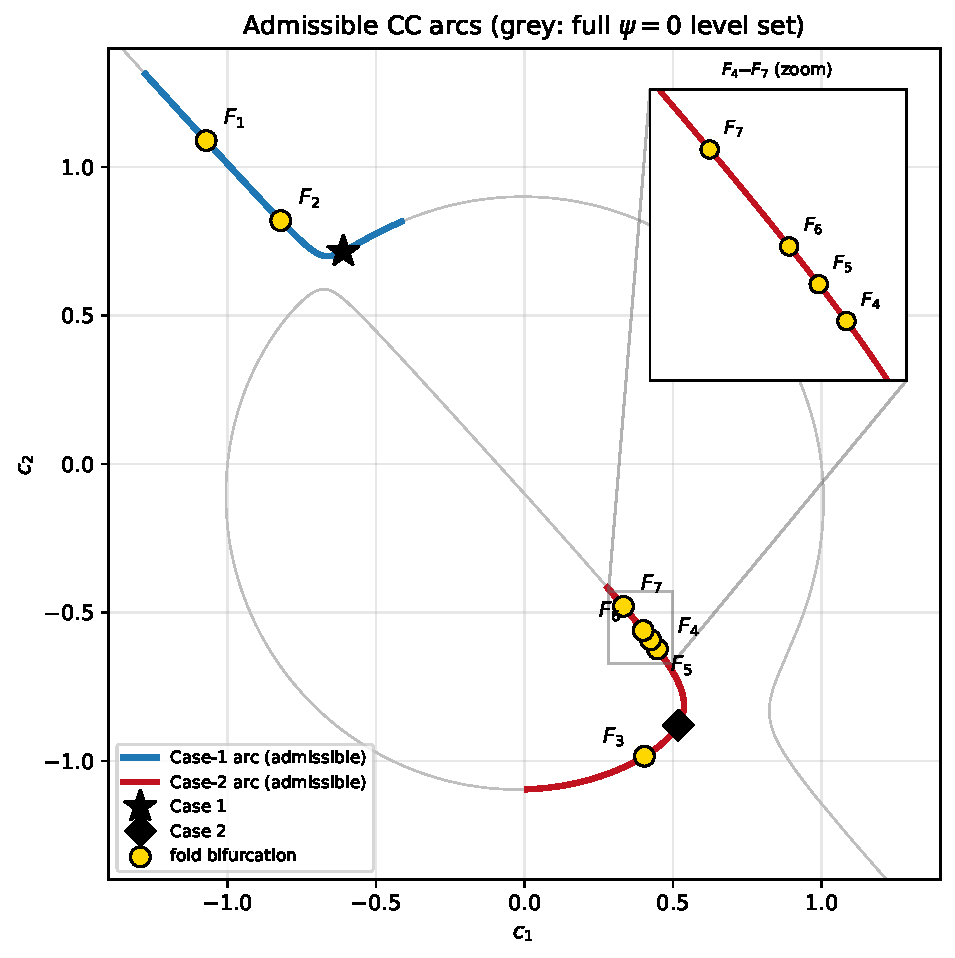
\includegraphics[width=0.72\textwidth]{cc_continuation_path.pdf}
\caption{Central-configuration branches and admissible arcs in the
$(c_1,c_2)$ plane at $(a,b)=(0.9,-0.1)$. Grey shows the numerically
represented $\psi=0$ branches in the plotted domain; blue and red denote
the admissible arcs containing Cases~1 and~2, respectively. Case~1 is
marked by a star and Case~2 by a diamond. Gold circles mark the seven
verified interior saddle-node folds $F_1$--$F_7$; the inset resolves the
closely spaced folds $F_4$--$F_7$. The two reference configurations lie
on distinct fixed-slice components, and each admissible arc terminates
where a primary mass ratio vanishes.}
\label{fig:cc_arcs}
\end{figure}


\subsection{Fold cascades and the eleven-equilibrium regime}
\label{subsec:cascades}

The equilibrium multiplicity cannot be determined by continuing only the
branches already known at a reference configuration, because a pair born
at a saddle-node does not exist on the opposite side of its fold. We
therefore use the independent multi-start search described in
Section~\ref{subsec:continuation} at every accepted central-configuration sample.

The resulting multiplicity function $N_{\rm eq}(s)$ is shown in
Figure~\ref{fig:count_staircase}. Along the two admissible arcs we obtain
\begin{equation}
\begin{aligned}
\text{Case-1 arc:}&\qquad
5\rightarrow7\rightarrow5\rightarrow4,
\\
\text{Case-2 arc:}&\qquad
7\rightarrow9\rightarrow11\rightarrow9\rightarrow7\rightarrow5.
\end{aligned}
\label{eq:count_cascades}
\end{equation}

The seven interior changes all have magnitude two and are subsequently
verified as generic saddle-node folds. They are denoted
$F_1,\ldots,F_7$ in Figures~\ref{fig:cc_arcs}--\ref{fig:count_staircase}
and listed in Table~\ref{tab:bifurcations}.

The final $5\rightarrow4$ change on the Case-1 arc is qualitatively
different. It occurs near
\[
s\simeq0.974
\]
as $\rho_2\rightarrow0$, when the underlying positive-mass primary
configuration approaches the boundary of the admissible set and an
associated equilibrium recedes to large distance. This is therefore a
mass-vanishing parameter-boundary degeneration, not an interior
saddle-node bifurcation. More generally, the admissible CC arcs terminate
when one of the primary mass ratios vanishes, but such arc termination must
not be conflated with an interior bifurcation of the restricted equilibrium
equations.

The local primary searches of Section~\ref{subsec:continuation} are especially important near
these limits, where equilibria associated with a small primary mass can lie
close to the corresponding singularity. The multiplicities in
\eqref{eq:count_cascades} are those obtained after applying the augmented
global-plus-local search throughout the arcs.

\begin{figure}[htbp]
\centering
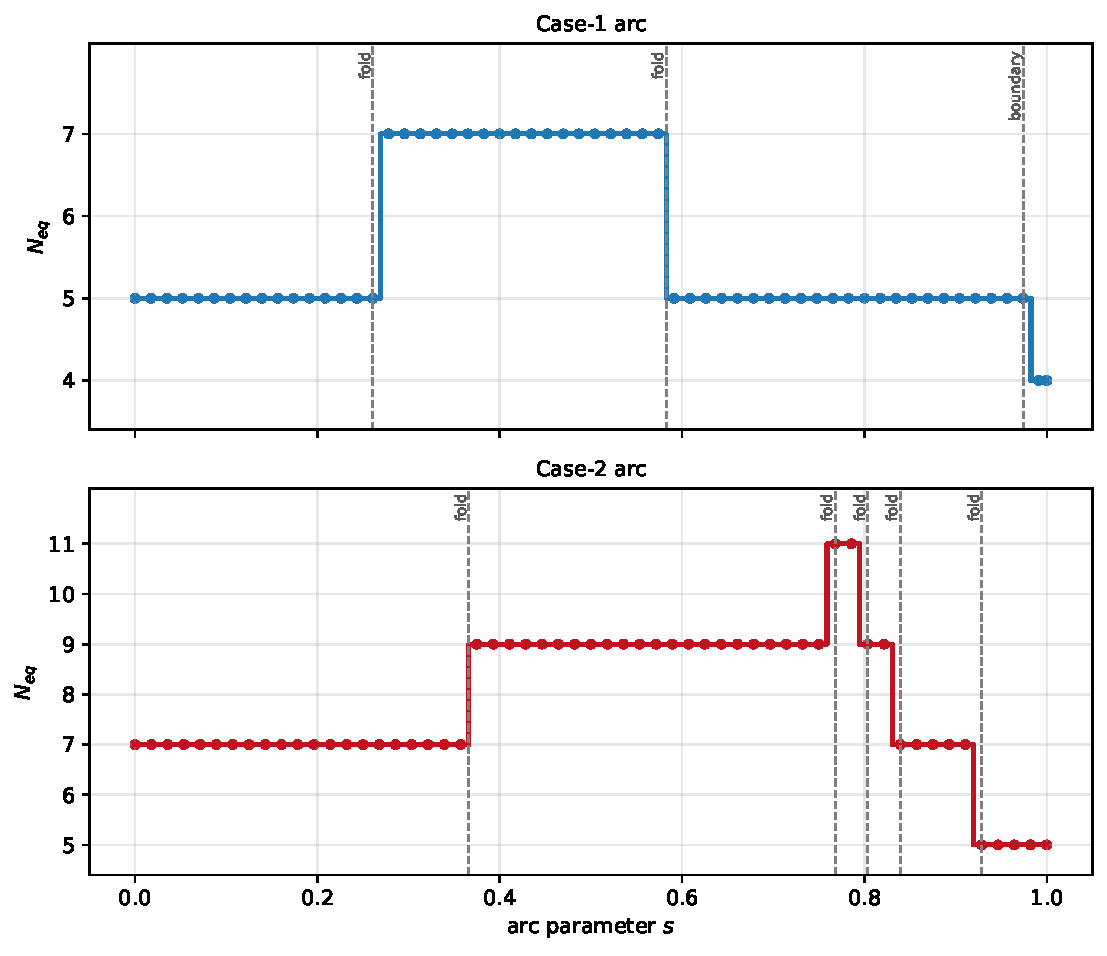
\includegraphics[width=\textwidth]{equilibrium_count_vs_s.pdf}
\caption{Equilibrium multiplicity $N_{\rm eq}(s)$ along the admissible
arcs. Top: Case-1 arc; bottom: Case-2 arc. Dashed vertical lines mark the
verified saddle-node folds $F_1$--$F_7$. The right-most Case-1 transition
is the mass-vanishing event $\rho_2\rightarrow0$ and is not an interior
fold.}
\label{fig:count_staircase}
\end{figure}


\begin{table}[t]
\centering
\footnotesize
\setlength{\tabcolsep}{4pt}
\caption{Verified changes in equilibrium multiplicity along the two
admissible central-configuration arcs. Interior count changes are generic
saddle-node folds located from
$\Omega_x=\Omega_y=\det H_\Omega=\psi=0$ and satisfying the
nondegeneracy conditions of Section~\ref{subsec:foldmethods}. The coordinates
$(c_1,c_2)_c$ describe the critical \emph{primary configuration};
$(\alpha,\beta)$ are the transversality and quadratic-nondegeneracy
coefficients of \eqref{eq:fold_coefficients}. The Case-1
$5\rightarrow4$ event is a mass-vanishing boundary degeneration rather
than an interior fold.}
\label{tab:bifurcations}
\begin{tabular}{llcccccl}
\hline
Arc & $N_{\rm eq}$ & Fold & $s_c$ &
$(c_1,c_2)_c$ & $(\rho_0,\rho_1,\rho_2)_c$ &
$(\alpha,\beta)$ & Type\\
\hline

Case-1 &
$5\to7$ &
$F_1$ &
0.261 &
$(-1.0717,1.0890)$ &
$(0.507,0.993,0.965)$ &
$(-2.72,22.4)$ &
saddle-node\\

Case-1 &
$7\to5$ &
$F_2$ &
0.583 &
$(-0.8206,0.8193)$ &
$(3.95,1.78,1.65)$ &
$(16.3,42.6)$ &
saddle-node\\

Case-1 &
$5\to4$ &
n/a &
0.974 &
n/a &
n/a &
n/a &
$\rho_2\to0$ boundary\\

Case-2 &
$7\to9$ &
$F_3$ &
0.366 &
$(0.4040,-0.9842)$ &
$(8.9,0.667,1.27)$ &
$(-0.615,0.0566)$ &
saddle-node\\

Case-2 &
$9\to11$ &
$F_4$ &
0.768 &
$(0.4478,-0.6231)$ &
$(0.71,2.19,2.28)$ &
$(-18.8,43.4)$ &
saddle-node\\

Case-2 &
$11\to9$ &
$F_5$ &
0.804 &
$(0.4246,-0.5923)$ &
$(0.576,2.49,2.57)$ &
$(1.18,0.231)$ &
saddle-node\\

Case-2 &
$9\to7$ &
$F_6$ &
0.839 &
$(0.3998,-0.5606)$ &
$(0.456,2.87,2.94)$ &
$(-6.03,-48.8)$ &
saddle-node\\

Case-2 &
$7\to5$ &
$F_7$ &
0.929 &
$(0.3333,-0.4795)$ &
$(0.189,4.3,4.35)$ &
$(0.506,0.173)$ &
saddle-node\\

\hline
\end{tabular}
\end{table}


\subsubsection{The eleven-equilibrium regime}
\label{subsubsec:eleven}

The most pronounced multiplicity increase occurs on the Case-2 arc. The
$9\rightarrow11$ fold $F_4$ at
\[
s_c\simeq0.768
\]
and the $11\rightarrow9$ fold $F_5$ at
\[
s_c\simeq0.804
\]
bound a narrow interval in which eleven distinct restricted equilibria are
detected. The two folds occur at different primary configurations
(Table~\ref{tab:bifurcations}) and at spatially separated restricted
equilibria. They are therefore two distinct saddle-node events rather than
a single higher-codimension degeneracy.

Tracking the individual branches through this interval reveals a feature
that is not visible from the multiplicity alone. At $F_4$, a new pair,
denoted $B_a$, is created near the critical restricted equilibrium
\[
(x,y)\simeq(-0.38,\,0.31).
\]
At the representative point
\[
s\simeq0.786
\]
inside the eleven-equilibrium interval, its two members lie approximately
at
\[
(-0.439,\,0.377),
\qquad
(-0.301,\,0.218).
\]

The pair destroyed at the subsequent $11\rightarrow9$ fold $F_5$ is not
$B_a$. Instead, $F_5$ annihilates a pre-existing pair, denoted $B_b$, in
the lower part of the equilibrium configuration near
\[
(x,y)\simeq(0.53,\,-1.70).
\]
Immediately before the fold its two members lie approximately at
\[
(0.26,\,-1.74),
\qquad
(0.74,\,-1.64).
\]
Branch tracking shows that this pair was created earlier at the
$7\rightarrow9$ fold $F_3$.

The newly created pair $B_a$ therefore survives the
$11\rightarrow9$ transition and remains present throughout the following
nine-equilibrium interval. It is annihilated only at $F_6$, the subsequent
$9\rightarrow7$ fold near
\[
(x,y)\simeq(-0.26,\,0.12).
\]
Consequently,
\[
9\rightarrow11\rightarrow9
\]
is not a simple creation and subsequent destruction of the same equilibrium
pair. The two nine-equilibrium intervals on either side of the
eleven-equilibrium window have the same multiplicity but different branch
populations. The eleven-equilibrium interval therefore exhibits a genuine
branch exchange.

As a robustness check, the equilibrium search was repeated at the
representative point
\[
s\simeq0.786,
\qquad
(c_1,c_2)\simeq(0.432,-0.602),
\]
inside the eleven-equilibrium interval.
The re-search uses the same $81\times81$ deterministic grid over
$[-8,8]^2$ and the same $35\times35$ local grid around each primary as the
main continuation analysis, but increases the number of fixed-seed random
starts from 1000 to 1500 (seed 20260808). It again returns eleven distinct
equilibria. Every retained root satisfies
\[
\|\nabla\Omega\|<10^{-12}.
\]
The minimum pairwise separation among all eleven roots at this configuration
is approximately
\[
0.175,
\]
while the separation of the two members of the newly created pair $B_a$ is
approximately
\[
0.21.
\]

We therefore report eleven as the number of distinct equilibria detected
under the stated numerical search procedure. This is a numerically supported
multiplicity on the investigated parameter interval; it is not an analytic
upper bound on the number of real equilibria of the general restricted
five-body problem.

This count is stable under refinement of the search. Repeating the multi-start
search at the eleven-equilibrium configuration over grid densities $61^2$
through $121^2$, random-start counts from $1000$ to $4000$, and three
independent seeds returns eleven equilibria in every case. Reducing the
converged-root rejection radius from $10^{-2}$ through $5\times10^{-3}$ to
$10^{-3}$ reveals no additional roots, and the closest equilibrium to any
primary at this configuration lies at distance $0.33$, so no genuine
near-primary equilibrium is discarded by the exclusion guard. The same
invariance holds for the four reference configurations, whose nearest
equilibrium-to-primary distance is $0.13$. These convergence and
exclusion-radius data are provided in the reproducibility archive.

Figure~\ref{fig:case2_cascade} shows representative equilibrium geometries
through the complete Case-2 sequence
\[
7\rightarrow9\rightarrow11\rightarrow9\rightarrow7\rightarrow5,
\]
with $B_a$ and $B_b$ identified explicitly. The radial branch representation
in Figure~\ref{fig:radial_branches} gives the complementary continuation
view and makes the branch exchange visible even where the scalar
multiplicity alone cannot distinguish branch identity.

\begin{figure}[htbp]
\centering
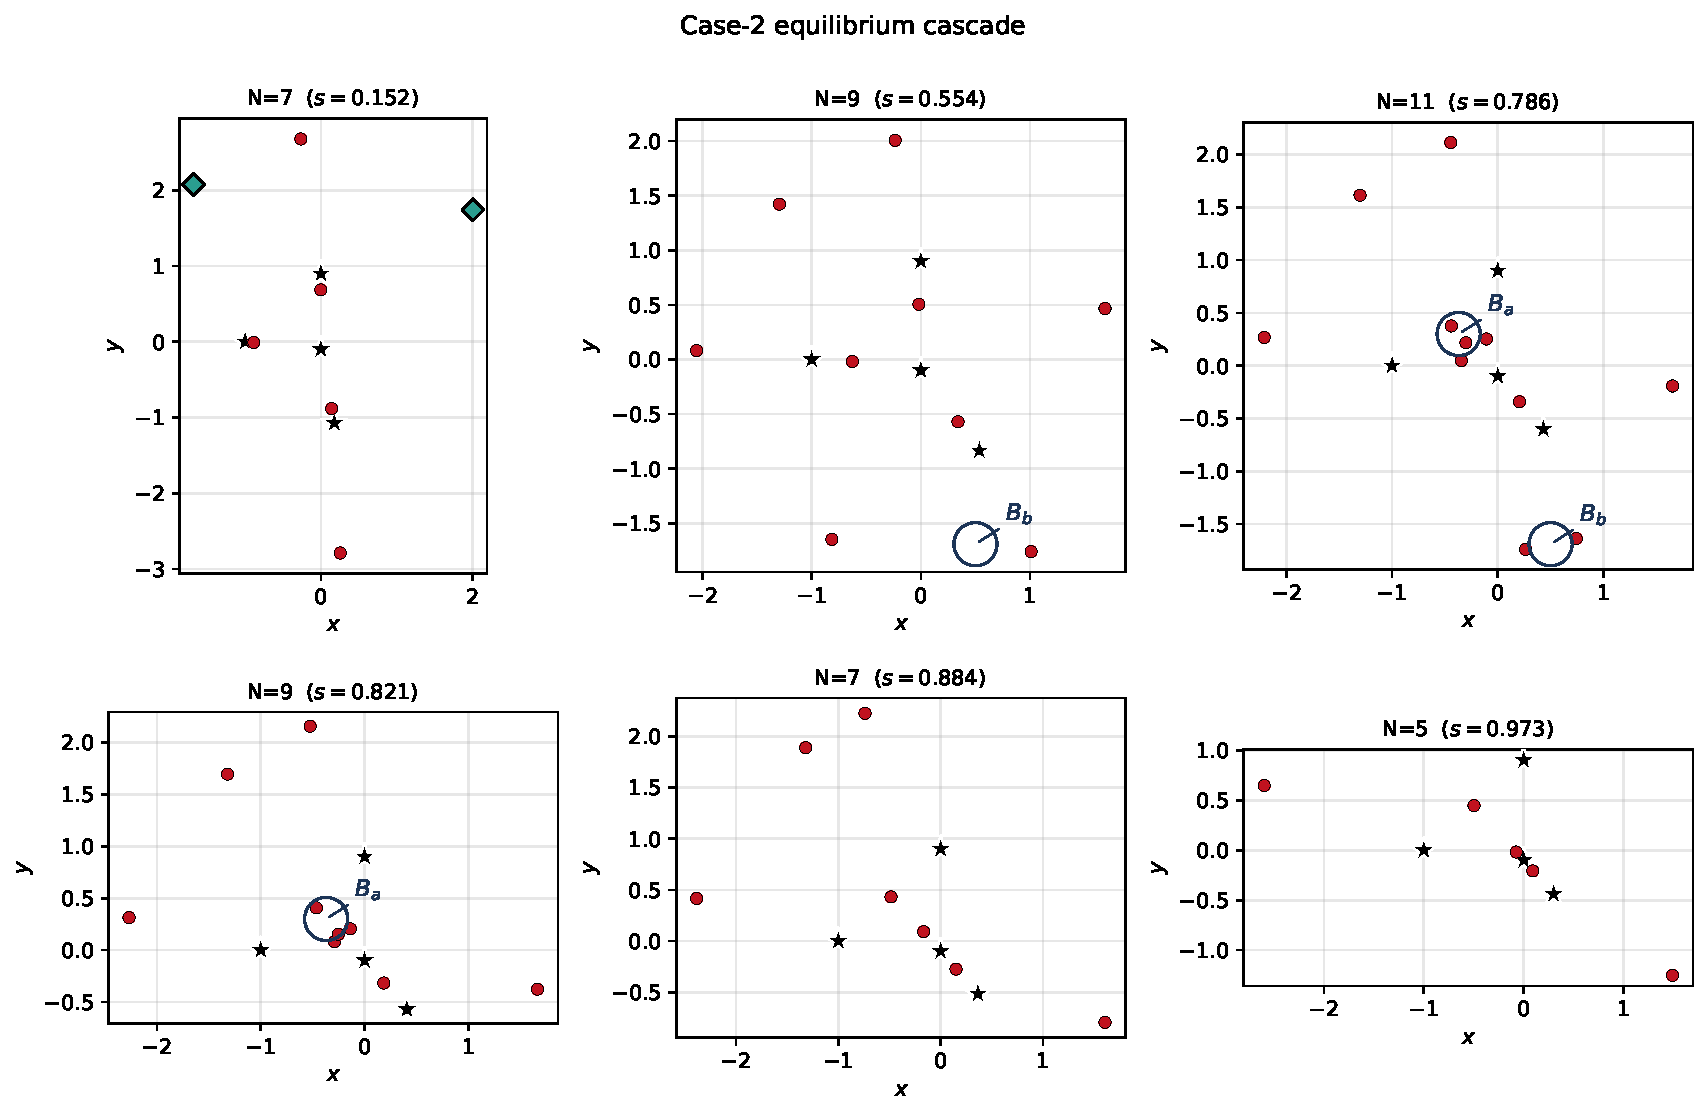
\includegraphics[width=\textwidth]{cascade_geometry_snapshots.pdf}
\caption{Equilibrium geometry at representative points of the Case-2
cascade $7\rightarrow9\rightarrow11\rightarrow9\rightarrow7
\rightarrow5$. Stars denote primaries, red circles unstable equilibria,
and green diamonds spectrally stable equilibria. The branch exchange in
the eleven-equilibrium interval is annotated explicitly: $B_a$, created
at $F_4$, persists into the following $N_{\rm eq}=9$ interval, whereas
the pre-existing pair $B_b$ is destroyed at $F_5$.}
\label{fig:case2_cascade}
\end{figure}


The branch identities shown in Figure~\ref{fig:radial_branches} are those
obtained from the adaptive predictor-based tracker of Section~\ref{subsec:continuation}. The same
branch assignment is used for the stability, centre-frequency, Jacobi, and
periodic-orbit analyses that follow. Ordinary equilibrium branches are
therefore shown without individual labels, while the dynamically important
pairs $B_a$ and $B_b$ are highlighted explicitly. Large-radius excursions
near the ends of the admissible arcs correspond to equilibria receding as a
primary mass ratio approaches zero.

\begin{figure}[htbp]
\centering
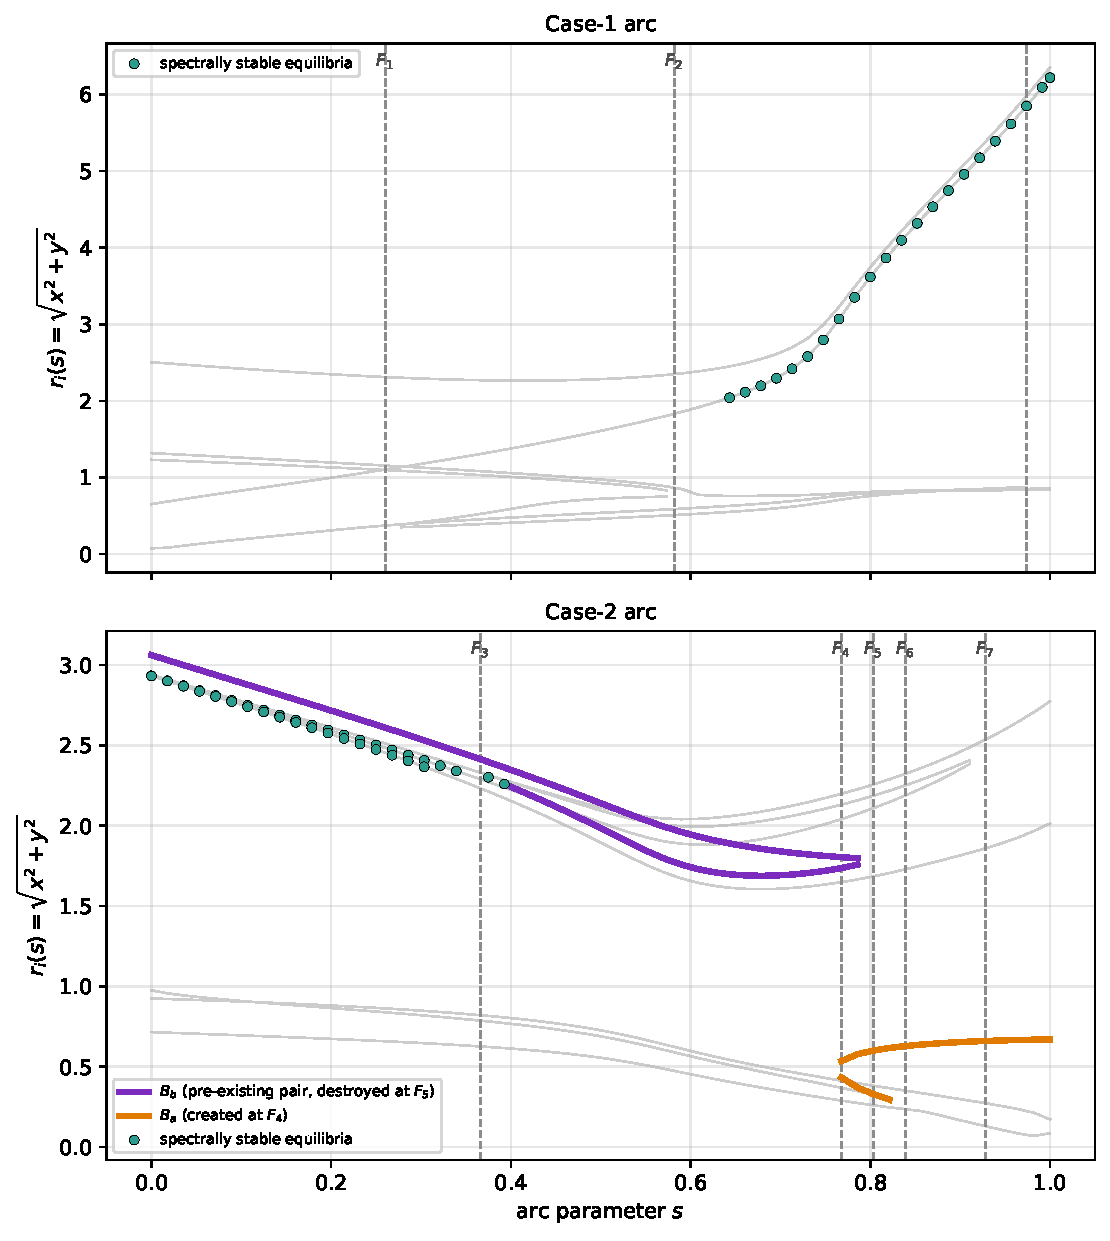
\includegraphics[width=\textwidth]{equilibrium_branches_r_vs_s.pdf}
\caption{Radial equilibrium coordinate
$r_i(s)=\sqrt{x_i(s)^2+y_i(s)^2}$ along the two admissible arcs.
Ordinary branches are shown in muted grey and dashed vertical lines mark
folds $F_1$--$F_7$. Spectrally stable equilibria are highlighted as
described in Section~\ref{sec:stability}. On the Case-2 arc, $B_a$ is the pair created at
$F_4$, whereas $B_b$ is the pre-existing pair destroyed at $F_5$,
directly displaying the branch exchange in the eleven-equilibrium
interval. Large-radius excursions near the arc ends correspond to
equilibria receding at mass-vanishing limits.}
\label{fig:radial_branches}
\end{figure}


\subsection{Saddle-node verification and scaling}
\label{subsec:foldverify}

The seven interior multiplicity changes in
\eqref{eq:count_cascades} are tested using the fold criteria of
Section~\ref{subsec:foldmethods}. For every transition, the augmented system
\begin{equation}
\Omega_x=\Omega_y=\det H_\Omega=\psi=0
\label{eq:fold_conditions_results}
\end{equation}
converges to a distinct critical point with augmented-system residual not
exceeding $10^{-11}$.

At each critical point the Hessian has one numerically vanishing eigenvalue,
denoted $\mu_0$, and one nonzero transverse eigenvalue, denoted
$\mu_\perp$. The corresponding transversality and
quadratic-nondegeneracy coefficients satisfy
\[
\alpha\neq0,
\qquad
\beta\neq0
\]
for all seven folds, with the computed $(\alpha,\beta)$ values listed in
Table~\ref{tab:bifurcations}. Thus every interior count change satisfies the
numerical conditions for a simple generic saddle-node fold.

The local branch geometry provides an independent verification. For each
fold the merging pair is resolved on the side of the critical parameter on
which both equilibria exist. The two roots approach one another and meet at
the numerically determined fold location, as illustrated for representative
cases in Figure~\ref{fig:fold_local}.

We further fit their separation to
\begin{equation}
d\propto|\ell-\ell_c|^\gamma
\label{eq:measured_fold_scaling}
\end{equation}
using the innermost resolved points. Across the seven folds the fitted
exponents satisfy
\[
0.44\leq\gamma\leq0.52,
\]
consistent with the Lyapunov--Schmidt prediction
\[
\gamma=\frac{1}{2}
\]
derived in Section~\ref{subsec:foldmethods}. Since the normalized coordinate $s$ is a smooth
monotone rescaling of $\ell$ on each admissible arc, the same local exponent
is obtained when the distance to the critical point is expressed using
$|s-s_c|$.

The agreement of four independent diagnostics (the observed
$\Delta N_{\rm eq}=\pm2$ count changes, convergence of the augmented
degeneracy system, satisfaction of the fold nondegeneracy conditions, and
the square-root pair-separation law) provides mutually consistent evidence
that $F_1,\ldots,F_7$ are generic saddle-node bifurcations of the restricted
equilibrium equations.

\begin{figure}[htbp]
\centering
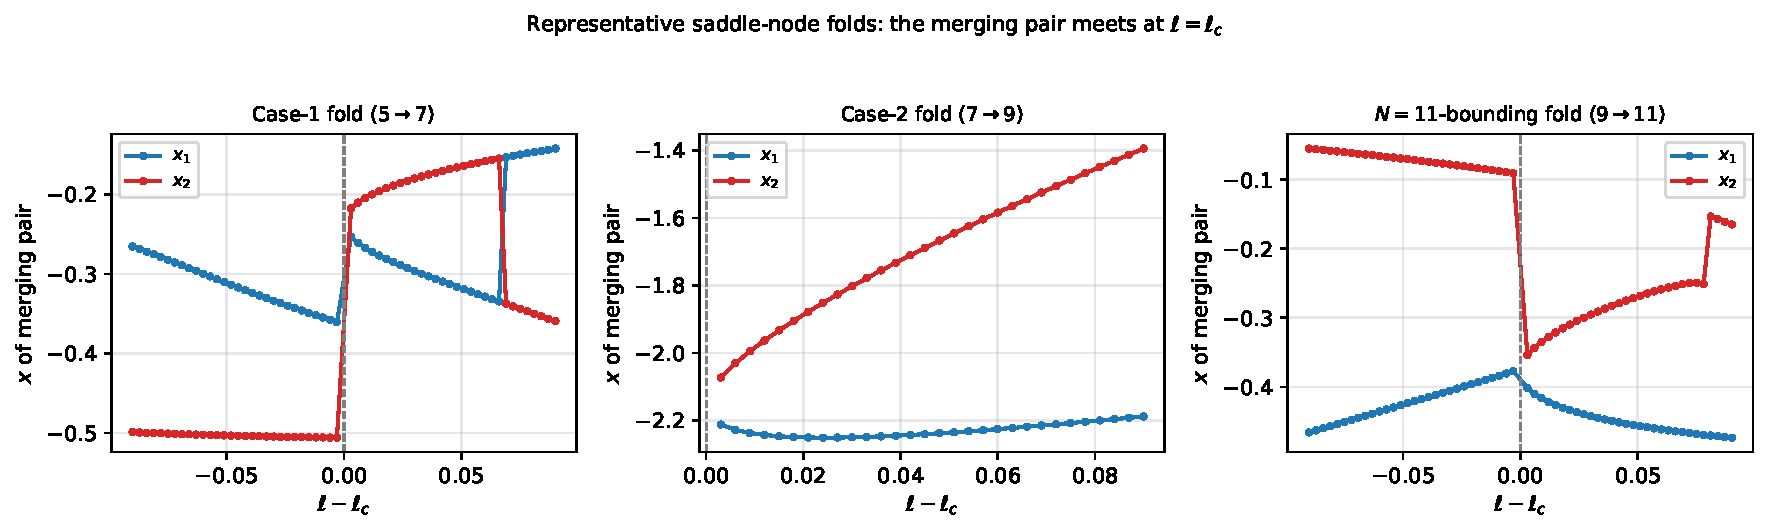
\includegraphics[width=\textwidth]{fold_zoom_main.pdf}
\caption{Three representative saddle-node folds (a Case-1 fold, an
ordinary Case-2 fold, and the $9\rightarrow11$ fold bounding the
eleven-equilibrium interval): the $x$-coordinates of the merging pair meet
at $\ell=\ell_c$ (dashed).}
\label{fig:fold_local}
\end{figure}

\begin{figure}[htbp]
\centering
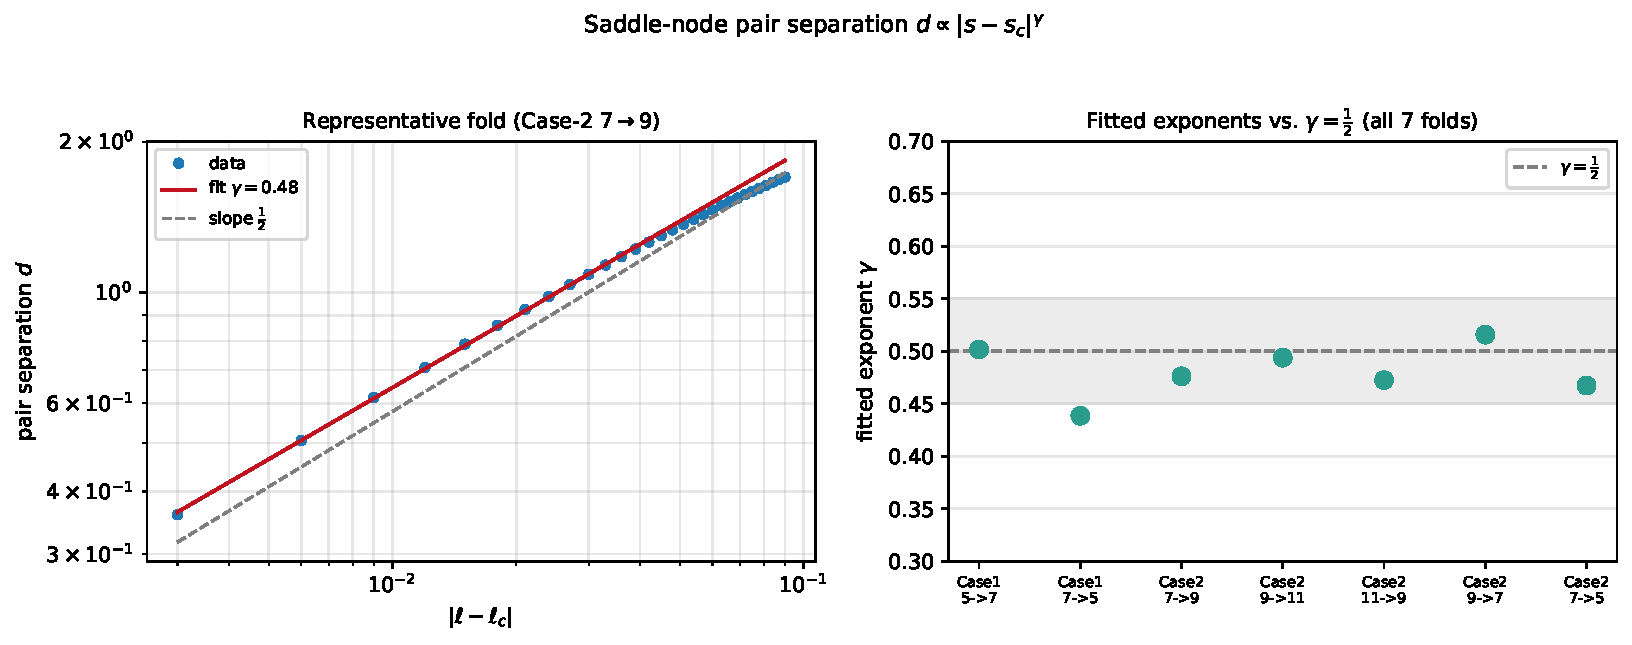
\includegraphics[width=0.78\textwidth]{fold_separation_exponent.pdf}
\caption{Saddle-node pair-separation scaling. Left: a representative fold
(Case-2 $7\rightarrow9$) showing the merging-pair separation $d$ against
$|\ell-\ell_c|$ on log--log axes, with the fitted slope and the reference
slope $\tfrac12$. Right: the fitted exponents $\gamma$ of all seven folds
against the theoretical value $\gamma=\tfrac12$ (shaded band
$[0.45,0.55]$); all lie in $[0.44,0.52]$.}
\label{fig:fold_scaling}
\end{figure}
\section{Stability and centre modes}
\label{sec:stability}

We now examine the linear stability of the equilibrium branches obtained in
Section~\ref{sec:results} and identify the centre modes from which the periodic-orbit
families of Section~\ref{sec:periodic} are continued. The spectral criterion and numerical
threshold have already been defined in Sections~\ref{subsec:potential} and~\ref{subsec:eqsearch}; here we focus
on the resulting stable intervals, the evolution of their centre
frequencies, and the occurrence of low-order near-commensurabilities.


\subsection{Spectral stability along the equilibrium branches}

For each reliably tracked equilibrium branch we compute
\[
\sigma(s)
=
\max_j \operatorname{Re}\lambda_j,
\]
where $\lambda_j$ are the eigenvalues of the rotating-frame variational
matrix \eqref{eq:variational_matrix}. As in Section~\ref{subsec:eqsearch}, an equilibrium is
classified as spectrally stable when
\[
\sigma\leq10^{-8}
\]
and the spectrum consists numerically of two purely imaginary conjugate
pairs. This is a statement about linear spectral stability only and does not
imply nonlinear or KAM stability.

The continuation shows that spectral stability is not confined to isolated
reference configurations. On the Case-1 arc, one equilibrium branch is
reliably tracked as spectrally stable over
\[
s\in[0.643,\,0.835].
\]
This branch contains the outer stable equilibrium identified in
Section~\ref{subsec:verification}. Stable spectral classifications are also
obtained farther toward the mass-vanishing end of the arc, but branch
tracking in this rapidly escaping region is flagged unreliable by the
criterion of Section~\ref{subsec:continuation}; those points are therefore
not used for branch-dependent conclusions. At the refined Case-1
configuration its position is
approximately
\[
(x,y)=(2.671,\,2.622),
\]
and its spectrum is
\begin{equation}
\lambda=\pm0.9632\,i,
\qquad
\lambda=\pm0.2984\,i,
\label{eq:case1_stable_spectrum}
\end{equation}
with real parts at the level of machine precision.

The Case-2 arc contains a richer stability structure. Two distinct
equilibrium branches are spectrally stable over substantial and overlapping
parts of the arc (Figure~\ref{fig:sigma}). One remains stable from the beginning of the admissible
arc to approximately
\[
s=0.339,
\]
and passes through
\[
(x,y)\simeq(-1.70,\,1.96)
\]
near $s=0.196$. A second stable branch persists to approximately
\[
s=0.304
\]
and passes through
\[
(x,y)\simeq(2.06,\,1.55)
\]
at nearly the same value of $s$. Thus a single primary configuration can
support more than one spectrally stable libration point. Isolated
single-sample classifications farther along the Case-2 arc are not used to
define additional stable intervals.

The pairs genuinely created at the seven interior saddle-node folds are
spectrally unstable at the first resolved points away from their folds.
In particular, the pair $B_a$ created at $F_4$ in the
eleven-equilibrium regime acquires nonzero real eigenvalues immediately
after its creation. The stable branches described above are instead
pre-existing equilibrium branches whose spectra become purely imaginary
over finite parameter intervals.

\begin{figure}[htbp]
\centering
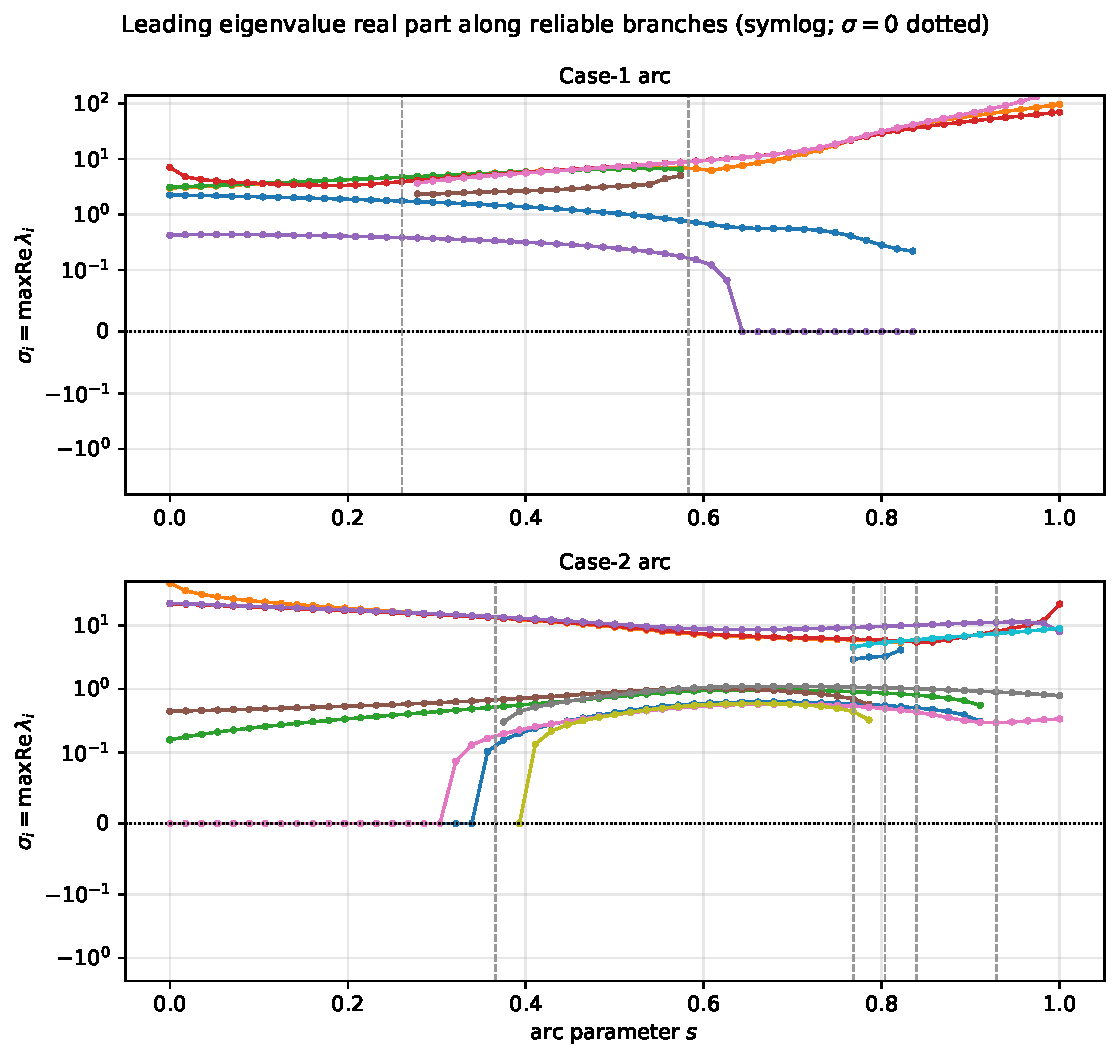
\includegraphics[width=\textwidth]{sigma_max_re_vs_s.pdf}
\caption{Leading eigenvalue real part $\sigma_i(s)$ along the reliably
tracked equilibrium branches. Dashed vertical lines mark the saddle-node
folds. On the Case-1 arc one branch is reliably tracked as spectrally
stable over $s\simeq[0.643,0.835]$. On the Case-2 arc two distinct branches are
spectrally stable, extending approximately to $s=0.339$ and $s=0.304$,
respectively. Spectral stability means that both eigenvalue pairs are
purely imaginary to the numerical threshold of Section~\ref{subsec:eqsearch}.}
\label{fig:sigma}
\end{figure}


\subsection{Centre frequencies and low-order near-commensurabilities}
\label{subsec:centrefreq}

At a doubly-elliptic equilibrium the spectrum has the form
\[
\lambda=\pm i\omega_1,
\qquad
\lambda=\pm i\omega_2,
\qquad
\omega_1\geq\omega_2>0.
\]
We follow both positive centre frequencies along each reliably stable
branch and examine the ratio
\[
R(s)=\frac{\omega_1(s)}{\omega_2(s)}.
\]
A point is flagged as a low-order near-commensurability when $R(s)$ lies
within $0.04$ of one of
\[
1,\quad
\frac{3}{2},\quad
2,\quad
\frac{5}{2},\quad
3,\quad
4.
\]
These flags are numerical proximity indicators only. They do not establish
an exact resonance or a nonlinear resonant bifurcation.

On the reliably tracked Case-1 stable branch, one low-order
near-commensurability is resolved (Figure~\ref{fig:ratio}). Near
\[
s\simeq0.678
\]
the equilibrium is approximately
\[
(x,y)\simeq(2.062,-0.756),
\]
with
\[
\omega_1\simeq0.8509,
\qquad
\omega_2\simeq0.5645,
\qquad
\frac{\omega_1}{\omega_2}\simeq1.5075,
\]
placing it within $0.0075$ of the $3{:}2$ ratio.

The two stable Case-2 branches exhibit different frequency-ratio
structures. On the branch passing through
\[
(x,y)\simeq(-1.70,\,1.96)
\]
at $s\simeq0.196$, the centre frequencies are
\[
\omega_1\simeq0.9172,
\qquad
\omega_2\simeq0.3721,
\]
so that
\begin{equation}
\frac{\omega_1}{\omega_2}
\simeq2.465.
\label{eq:case2_5to2_ratio}
\end{equation}
This is within approximately $0.035$ of the $5{:}2$ ratio. No $2{:}1$
near-commensurability occurs on this branch.

The second stable Case-2 branch passes successively near several low-order
ratios:
\[
\begin{array}{ccl}
s\simeq0.018
&:&
\omega_1/\omega_2\simeq3.995
\quad (4{:}1),
\\[1mm]
s\simeq0.125
&:&
\omega_1/\omega_2\simeq2.510
\quad (5{:}2),
\\[1mm]
s\simeq0.196
&:&
\omega_1/\omega_2\simeq1.983
\quad (2{:}1),
\\[1mm]
s\simeq0.268
&:&
\omega_1/\omega_2\simeq1.488
\quad (3{:}2).
\end{array}
\]
At the genuine Case-2 $2{:}1$ near-commensurability the equilibrium lies
near
\[
(x,y)\simeq(2.06,\,1.55),
\]
with
\[
\omega_1\simeq0.8933,
\qquad
\omega_2\simeq0.4506.
\]
The occurrence of two different stable equilibria at essentially the same
arc parameter $s\simeq0.196$ is important: one lies near $5{:}2$ and the
other near $2{:}1$. The arc parameter alone therefore does not uniquely
identify the dynamical state; branch identity must also be retained.

The periodic-orbit dataset of Section~\ref{sec:periodic} samples selected members of this
near-commensurate structure rather than attempting an exhaustive resonance
survey. Families~7--8 are continued from the Case-1 equilibrium near the
$3{:}2$ ratio. Families~9--10 are continued from the first Case-2 stable
branch, namely the equilibrium near
\[
(-1.70,\,1.96)
\]
whose frequency ratio is approximately $2.465$ and is therefore associated
with the $5{:}2$ near-commensurability. The distinct Case-2 equilibrium
near the $2{:}1$ ratio is not used as a parent in the present
periodic-orbit dataset.

\begin{figure}[htbp]
\centering
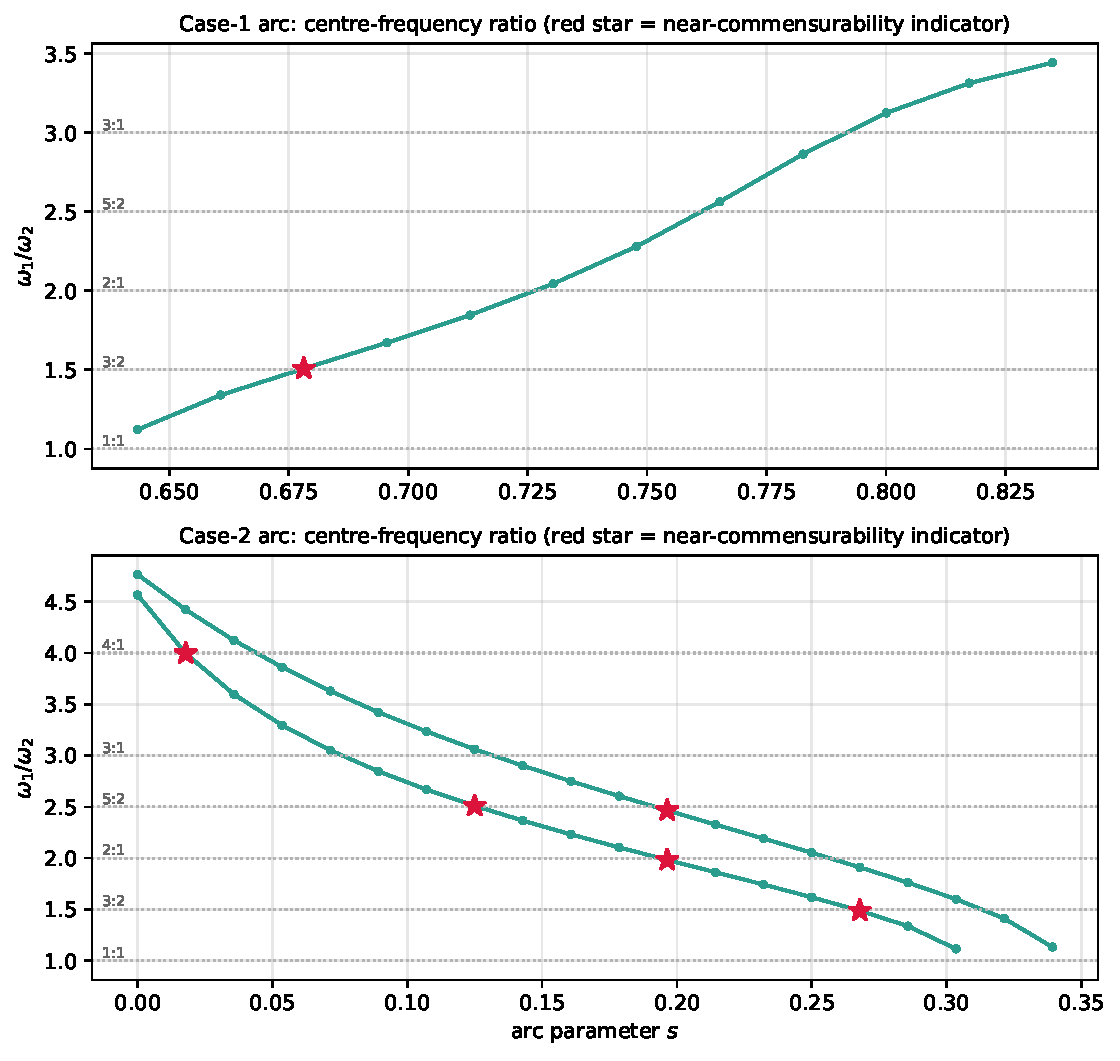
\includegraphics[width=\textwidth]{frequency_ratio_vs_s.pdf}
\caption{Centre-frequency ratio $\omega_1/\omega_2$ along the reliably
resolved spectrally stable branches. Dotted horizontal lines mark selected
low-order rational ratios, and highlighted points indicate proximity
within the tolerance $0.04$. These points are near-commensurability
indicators only and do not establish exact resonance. The Case-2 panel
contains two distinct stable equilibrium branches; at $s\simeq0.196$ one
lies near $5{:}2$ and the other near $2{:}1$.}
\label{fig:ratio}
\end{figure}


\subsection{Lyapunov-centre interpretation}
\label{subsec:lyapunov}

The centre modes identified above provide the local seeds for the
periodic-orbit families of Section~\ref{sec:periodic}. It is therefore useful to state
precisely when the Lyapunov centre theorem applies.

Let $\pm i\omega_k$ be the simple centre pair selected for continuation at
a parent equilibrium. The local Lyapunov family exists provided no other
eigenvalue of the variational matrix is an integer multiple
\[
\pm m i\omega_k,
\qquad
m=2,3,\ldots
\]
of that selected frequency. This condition is satisfied at every parent
used for the ten periodic-orbit families computed in Section~\ref{sec:periodic}.

For the saddle$\times$centre parents of families~5--6, the companion
eigenvalue pair is real. It therefore cannot equal an integer multiple of
the purely imaginary centre frequency. The hyperbolic direction makes the
resulting periodic families unstable, but it does not obstruct their local
existence as Lyapunov families.

For the doubly-elliptic parents, proximity to a rational frequency ratio
must be distinguished from exact resonance. In particular, the
Case-1 parent of families~7--8 has
\[
\omega_1/\omega_2\simeq1.5075,
\]
near but not equal to $3{:}2$, while the Case-2 parent of families~9--10 has
\[
\omega_1/\omega_2\simeq2.465,
\]
near but not equal to $5{:}2$. Neither ratio violates the exact
non-resonance hypothesis of the theorem. The same distinction applies to
the other near-commensurabilities identified above: numerical proximity to
$2{:}1$ or $4{:}1$ is not an exact integer resonance.

Accordingly, all ten families computed in Section~\ref{sec:periodic} are Lyapunov families
in the local theorem sense. What differs among them is the stability type
of the parent equilibrium and the proximity of its centre frequencies to
low-order commensurabilities. Whether a continued family subsequently
encounters a resonant or period-doubling bifurcation is a global
continuation question and must be decided from its Floquet multipliers
rather than inferred from the linear frequency ratio alone.
\section{Periodic-orbit families}
\label{sec:periodic}

The centre modes identified in Section~\ref{subsec:centrefreq} provide
local seeds for Lyapunov families of periodic orbits. We compute ten such
families, chosen to sample doubly-elliptic equilibria, saddle$\times$centre
equilibria, and selected low-order near-commensurability regions. This
section describes the shooting formulation and continuation procedure,
classifies the corrected orbits by their Floquet multipliers, and examines
the approach of two families to the period-doubling threshold. The computed
families are summarized in Table~\ref{tab:periodic_families}.

% AUTO-GENERATED by paper/make_tables.py from results/*.csv. Do not edit by hand.
\begin{table}[t]
\centering
\caption{Computed periodic-orbit families. Each family is a Lyapunov family seeded from a simple centre mode of a parent equilibrium and continued in amplitude; the Lyapunov centre theorem applies at every parent (the exact non-resonance condition holds, including at the saddle$\times$centre parents of families 5--6 and the near-resonant parents of families 7--10; see Section~\ref{subsec:lyapunov}). What differs is the parent stability type and proximity to resonance, not theoretical standing. `mode' is the centre frequency $\omega$; $N$ the number of corrected members; the $C_J$ and $T$ ranges are over the family; `max closure' is the largest periodicity residual $\|u(T)-u_0\|$ attained over the family's members (all $<10^{-10}$). Floquet class is by the stability index $\nu$ ($|\nu|<2$ stable).}
\label{tab:periodic_families}
\footnotesize
\setlength{\tabcolsep}{3.5pt}
\begin{tabular}{clcccccl}
\toprule
Fam & parent (arc, eq.) & $\omega$ & $N$ & $C_J$ range & $T$ range & max closure & Floquet / note \\
\midrule
1 & Case-1 stable, $(2.78,0.25)$ & $0.925$ & 22 & $[23.89,24.03]$ & $[6.78,6.79]$ & $5.3\times10^{-11}$ & Floquet stable \\
2 & Case-1 stable, $(2.78,0.25)$ & $0.406$ & 20 & $[24.03,24.04]$ & $[15.48,15.52]$ & $8.1\times10^{-11}$ & Floquet stable \\
3 & Case-2 stable, $(1.99,1.79)$ & $0.922$ & 23 & $[21.34,21.79]$ & $[6.68,6.82]$ & $3.5\times10^{-11}$ & Floquet stable \\
4 & Case-2 stable, $(1.99,1.79)$ & $0.390$ & 20 & $[21.79,21.80]$ & $[16.13,16.51]$ & $4.1\times10^{-11}$ & Floquet stable \\
5 & Case-1 sdl$\times$ctr, $(-0.97,0.51)$ & $3.738$ & 18 & $[13.33,13.43]$ & $[1.68,1.72]$ & $7.6\times10^{-11}$ & real unstable \\
6 & Case-2 sdl$\times$ctr, $(0.35,-0.64)$ & $7.435$ & 15 & $[24.28,24.29]$ & $[0.85,0.85]$ & $8.6\times10^{-11}$ & real unstable \\
7 & Case-1 $3{:}2$ reg., $(2.06,-0.76)$ & $0.851$ & 20 & $[15.23,15.25]$ & $[7.38,7.38]$ & $6.0\times10^{-11}$ & Floquet stable \\
8 & Case-1 $3{:}2$ reg., $(2.06,-0.76)$ & $0.564$ & 21 & $[15.25,15.29]$ & $[11.13,11.39]$ & $1.7\times10^{-11}$ & Floquet stable; $\nu\!\to\!-2$ \\
9 & Case-2 $5{:}2$ reg., $(-1.70,1.96)$ & $0.917$ & 21 & $[20.28,20.36]$ & $[6.79,6.85]$ & $9.0\times10^{-11}$ & Floquet stable \\
10 & Case-2 $5{:}2$ reg., $(-1.70,1.96)$ & $0.372$ & 18 & $[20.36,20.36]$ & $[16.89,17.17]$ & $2.6\times10^{-11}$ & Floquet stable; $\nu\!\to\!-2$ \\
\bottomrule
\end{tabular}
\end{table}



\subsection{Shooting formulation and linear seeding}
\label{subsec:periodic_shooting}

Write the rotating-frame state as
\[
\mathbf u=(x,y,\dot{x},\dot{y})^T
\]
and denote by $\phi_T(\mathbf u_0)$ the time-$T$ flow of
\eqref{eq:equations_of_motion}. A periodic orbit satisfies
\begin{equation}
\phi_T(\mathbf u_0)-\mathbf u_0=\mathbf 0.
\label{eq:periodicity_residual}
\end{equation}

Let
\[
L_j=(x^\ast,y^\ast,0,0)^T
\]
be a parent equilibrium with a simple centre eigenvalue
$+i\omega_k$ and corresponding complex eigenvector $\mathbf w_k$ of the
variational matrix \eqref{eq:variational_matrix}. The small-amplitude
linear motion provides the initial approximation
\[
\mathbf u(t)
=
L_j+
\varepsilon
\operatorname{Re}
\left(
e^{i\omega_k t}\mathbf w_k
\right).
\]
Using the real part of the selected eigenvector as the initial direction,
we take
\begin{equation}
\mathbf u_0^{(0)}
=
L_j+\varepsilon\widehat{\mathbf e}_k,
\qquad
\widehat{\mathbf e}_k
=
\frac{\operatorname{Re}\mathbf w_k}
{\|\operatorname{Re}\mathbf w_k\|},
\qquad
T_0=\frac{2\pi}{\omega_k}.
\label{eq:linear_periodic_seed}
\end{equation}
At a doubly-elliptic equilibrium the two simple centre modes are seeded
separately, producing two local Lyapunov families.

The periodicity equations alone do not isolate a unique member of a
one-parameter family because the autonomous flow also admits arbitrary
time translation along a periodic orbit. We therefore supplement the four
periodicity equations with a phase condition and an amplitude condition,
\begin{equation}
\widehat{\mathbf e}_k^T f(\mathbf u_0)=0,
\qquad
\widehat{\mathbf e}_k^T(\mathbf u_0-L_j)=a,
\label{eq:phase_amplitude_conditions}
\end{equation}
where $f$ denotes the rotating-frame vector field and $a$ is the prescribed
continuation amplitude.

The complete correction residual is consequently
\begin{equation}
\mathcal R(\mathbf u_0,T)=
\begin{pmatrix}
\phi_T(\mathbf u_0)-\mathbf u_0\\
\widehat{\mathbf e}_k^T f(\mathbf u_0)\\
\widehat{\mathbf e}_k^T(\mathbf u_0-L_j)-a
\end{pmatrix}.
\label{eq:shooting_residual}
\end{equation}
The state-transition matrix $\Phi(t)$ is integrated simultaneously from
\[
\dot{\Phi}=A(\mathbf u(t))\Phi,
\qquad
\Phi(0)=I,
\]
and the monodromy matrix is
\[
M=\Phi(T).
\]
The derivatives of the periodicity residual are
\[
D_{\mathbf u_0}
\bigl[\phi_T(\mathbf u_0)-\mathbf u_0\bigr]
=
M-I,
\qquad
D_T
\bigl[\phi_T(\mathbf u_0)-\mathbf u_0\bigr]
=
f(\phi_T(\mathbf u_0)).
\]
Thus the $6\times5$ correction Jacobian is
\begin{equation}
J=
\begin{pmatrix}
M-I & f(\phi_T(\mathbf u_0))\\
\widehat{\mathbf e}_k^T A(\mathbf u_0) & 0\\
\widehat{\mathbf e}_k^T & 0
\end{pmatrix},
\label{eq:shooting_jacobian}
\end{equation}
and each Newton correction is obtained from the least-squares problem
\[
\delta X
=
\arg\min_{\delta}
\|J\delta+\mathcal R\|_2.
\]
The phase and amplitude constraints remove the two neutral directions
associated with time translation and displacement along the local
one-parameter family. The resulting overdetermined formulation retains all
four periodicity equations symmetrically rather than eliminating a state
coordinate through the Jacobi integral.


\subsection{Continuation and numerical validation}
\label{subsec:periodic_continuation}

The state, period, and state-transition matrix are integrated with DOP853
using
\[
\mathrm{rtol}=\mathrm{atol}=10^{-12}.
\]
Newton corrections are capped according to
\[
\|\delta\mathbf u_0\|\leq0.5,
\qquad
|\delta T|\leq0.5T,
\]
with $T>0$ enforced throughout.

A corrected orbit is accepted only when
\begin{equation}
\|\phi_T(\mathbf u_0)-\mathbf u_0\|_2<10^{-10},
\qquad
|\widehat{\mathbf e}_k^T f(\mathbf u_0)|<10^{-10},
\qquad
|\widehat{\mathbf e}_k^T(\mathbf u_0-L_j)-a|<10^{-12}.
\label{eq:periodic_acceptance}
\end{equation}
Across the 198 accepted periodic solutions the observed maxima are
\[
\|\phi_T(\mathbf u_0)-\mathbf u_0\|_2
\leq9.0\times10^{-11},
\]
\[
|\widehat{\mathbf e}_k^T f(\mathbf u_0)|
\leq4.7\times10^{-12},
\qquad
|\widehat{\mathbf e}_k^T(\mathbf u_0-L_j)-a|
\leq3.9\times10^{-16}.
\]
The periodicity residual therefore provides a direct numerical certificate
that every orbit reported below closes to the stated tolerance.

We continue each family using the natural amplitude parameter
\[
a=
\widehat{\mathbf e}_k^T(\mathbf u_0-L_j),
\]
with the prescribed amplitudes forming the geometric sequence
\begin{equation}
a_0=2\times10^{-3},
\qquad
a_{n+1}=1.35\,a_n.
\label{eq:amplitude_sequence}
\end{equation}
Each new member is predicted from its predecessor and then corrected by the
shooting system above, with at most 40 Newton iterations. For geometric
interpretation we also record
\[
A=
\max_t
\sqrt{(x(t)-x^\ast)^2+(y(t)-y^\ast)^2}.
\]

Several safeguards prevent continuation onto spurious or unrelated
solutions. Correction is terminated after an integration failure caused by
a near collision; solutions with
\[
T<0.4T_0
\]
are rejected to prevent collapse toward the trivial $T\rightarrow0$
solution; and the family is terminated if the geometric amplitude more than
doubles between consecutive members. Continuation also stops when the orbit
approaches a primary within $0.05$ or when
\[
A>2.5.
\]

Because the continuation parameter is the prescribed amplitude $a$, these
computations determine only the portion of each family reachable while $a$
remains a useful monotone local coordinate. We therefore make no claim that
the computed curves are maximal periodic-orbit families. Continuation
through a turning point in $a$ would require pseudo-arclength continuation
in the extended periodic-orbit system, which is not attempted here.

The ten parent modes were chosen to sample distinct dynamical situations.
Families~1--4 use both centre modes of one doubly-elliptic equilibrium on
each admissible arc. Families~5--6 use centre modes of selected
saddle$\times$centre equilibria. Families~7--8 are seeded from the
Case-1 equilibrium near the $3{:}2$ near-commensurability identified in
Section~\ref{subsec:centrefreq}, and families~9--10 from the distinct
Case-2 equilibrium near the $5{:}2$ near-commensurability. As established
in Section~\ref{subsec:centrefreq}, the latter parent is
\[
(x,y)\simeq(-1.70,1.96),
\qquad
\omega_1/\omega_2\simeq2.465,
\]
and is not the separate Case-2 equilibrium lying near the $2{:}1$ ratio.

For every family the smallest corrected members approach the intended
linear mode:
\[
\mathbf u_0(a)\rightarrow L_j,
\qquad
T(a)\rightarrow\frac{2\pi}{\omega_k}
\qquad\text{as }a\rightarrow0.
\]
For example,
\[
\frac{2\pi}{0.925}=6.793,\qquad
\frac{2\pi}{0.406}=15.48,\qquad
\frac{2\pi}{0.922}=6.815,
\]
in agreement with the smallest computed periods of families~1--3 to the
reported precision.


\subsection{Floquet stability}
\label{subsec:floquet}

The linear stability of each corrected periodic orbit is determined from
its monodromy matrix $M=\Phi(T)$. The Hamiltonian structure of the
rotating-frame problem implies reciprocal symmetry of the Floquet
multipliers. For a periodic orbit of this two-degree-of-freedom autonomous
Hamiltonian system there is also a trivial multiplier pair at $+1$,
associated with the flow and energy-family directions. Numerically this
pair is recovered to within a few times $10^{-6}$.

After removal of the trivial pair, one nontrivial reciprocal multiplier
pair remains. If its members are denoted $\lambda$ and $\lambda^{-1}$, we
use the stability index
\begin{equation}
\nu
=
\lambda+\lambda^{-1}.
\label{eq:floquet_index}
\end{equation}
For the planar problem $\nu$ is real. The nontrivial multipliers lie on the
unit circle when
\[
|\nu|<2
\]
and form a real reciprocal pair when
\[
|\nu|>2.
\]
The limiting values
\[
\nu=+2
\qquad\text{and}\qquad
\nu=-2
\]
correspond respectively to a $+1$ collision and a period-doubling
($-1$) collision of the nontrivial multipliers.

We use ``Floquet stable'' only to mean that the nontrivial multiplier pair
lies on the unit circle to the stated numerical tolerance; it does not
imply nonlinear stability of the periodic orbit. Since only one
nontrivial reciprocal pair remains in the planar problem, a Hamiltonian
collision between two distinct nontrivial multiplier pairs cannot occur;
the relevant local stability boundaries are therefore the values
$\nu=\pm2$.

Although DOP853 is not a symplectic integrator, the computed monodromy
matrices preserve the expected Hamiltonian structure to good numerical
accuracy. Over the 198 accepted orbits,
\[
|\det M-1|\leq1.5\times10^{-8},
\qquad
|\lambda_1\lambda_2-1|\leq1.5\times10^{-8},
\]
with median values near $10^{-13}$, while the trivial pair remains within
$5\times10^{-6}$ of $+1$ (median $\sim3\times10^{-8}$). These diagnostics
provide an independent numerical check on the Floquet classification.


\subsection{Computed families and near-period-doubling behaviour}
\label{subsec:periodic_results}

The ten families comprise 198 accepted periodic solutions. Their parent
equilibria, centre frequencies, Jacobi and period ranges, closure residuals,
and Floquet classifications are summarized in
Table~\ref{tab:periodic_families}.

Before turning to the individual families, it is useful to fix their
geometric character. Each parent equilibrium is a libration point of the
rotating four-primary configuration, and the associated Lyapunov orbits are
small oscillations \emph{about that point} rather than revolutions about any
individual primary. This is illustrated in Figure~\ref{fig:orbit_potential}.
For the Case-2 parent of family~3 the Hessian of $\Omega$ is positive
definite, with eigenvalues $0.0436$ and $2.9554$, so the parent is a strict
local minimum of the rotating-frame effective potential. It is also the
numerically identified global minimum of $2\Omega$ for this primary
configuration, with $2\Omega_{\min}\simeq21.7867$. The computed family
members satisfy $C_J\le2\Omega_{\min}$; consequently the corresponding
numerical Hill set contains no forbidden region and is the whole plane. The
nested family is therefore organized by the local potential minimum rather
than by confinement within a closed zero-velocity boundary.

\begin{figure}[htbp]
  \centering
  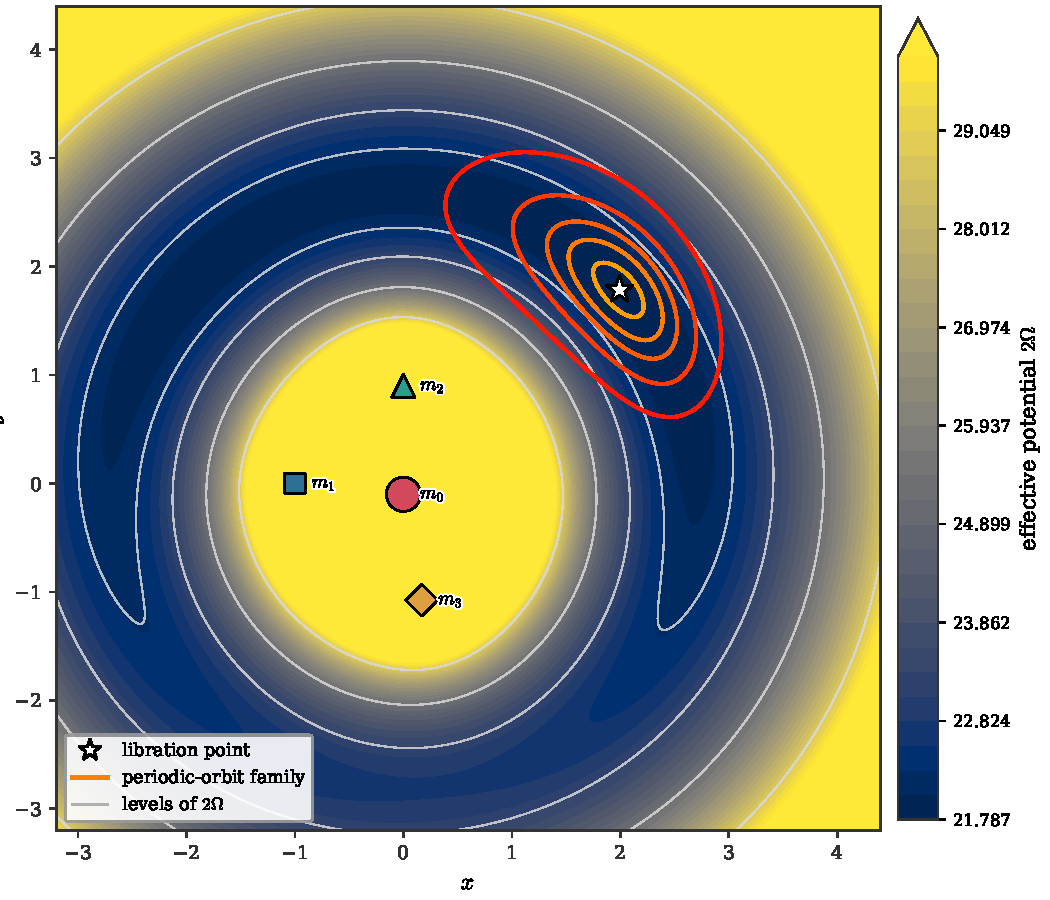
\includegraphics[width=0.8\textwidth]{periodic_orbit_potential.pdf}
  \caption{Effective-potential landscape for the Case-2 configuration
  supporting periodic-orbit family~3. Filled contours show $2\Omega(x,y)$,
  with the colour range clipped at large values for visualization;
  $2\Omega\to+\infty$ at the primary singularities and at large distance.
  Thin grey curves are representative level curves of $2\Omega$ at $22.29$,
  $23.29$, $25.29$, and $28.79$. The four primaries are marked by
  $m_0$--$m_3$, and the star denotes the doubly-elliptic parent equilibrium.
  The Hessian of $\Omega$ at this point has eigenvalues $0.0436$ and
  $2.9554$, so the parent is a strict local minimum of the effective
  potential. Successive members of the associated Lyapunov family are shown
  from small to larger amplitude, illustrating libration about the
  equilibrium of the rotating four-primary configuration rather than orbital
  motion about any individual primary.}
  \label{fig:orbit_potential}
\end{figure}

Families~1--4 originate from the selected doubly-elliptic equilibria on the
two admissible arcs. Both centre modes of each parent produce corrected
Lyapunov families whose nontrivial Floquet multipliers remain on the unit
circle throughout the computed intervals. Figures~\ref{fig:family_case1}
and~\ref{fig:family_case2} show representative small, intermediate, and
large members. The smallest solutions reproduce the corresponding linear
centre modes, while larger members deform substantially without losing
Floquet stability over the continuation range. Figure~\ref{fig:famevol}
shows the period, geometric amplitude, and Floquet index of all ten
families against $C_J$.

Families~5--6 demonstrate the contrasting behaviour of
saddle$\times$centre parents. Their selected centre modes satisfy the
Lyapunov-centre non-resonance condition discussed in
Section~\ref{subsec:centrefreq}, so genuine local periodic families exist
despite the hyperbolic companion direction. Their nontrivial Floquet
multipliers, however, form a strongly real reciprocal pair, giving
\[
|\nu|\sim10^3
\]
over the computed portions. These families are therefore real unstable.
A representative member is shown in Figure~\ref{fig:selected_orbits}.

Families~7--10 sample the near-commensurate doubly-elliptic regions.
Families~7--8 originate near the Case-1 $3{:}2$ ratio, while
families~9--10 originate near the Case-2 $5{:}2$ ratio. These ratios are
near-commensurabilities rather than exact resonances at the parent
equilibria, so their local existence as Lyapunov families is unaffected.

Two of these families approach the period-doubling boundary
$\nu=-2$ as their amplitudes increase. Fine continuation near the minimum
of
\[
|\nu+2|
\]
shows that family~8 remains approximately
\[
2\times10^{-3}
\]
away from the threshold, whereas family~10 approaches much more closely,
reaching
\begin{equation}
\min_a|\nu+2|
\simeq1.0\times10^{-7},
\qquad
\nu\simeq-1.99999990,
\qquad
A\simeq0.28.
\label{eq:near_period_doubling}
\end{equation}
The index subsequently moves away from $-2$ rather than crossing it
(Figure~\ref{fig:period_doubling_scan}).

The approach was re-examined with an ultra-fine amplitude sweep of $51$
samples spanning amplitudes $0.258$ to $0.298$ (step $8\times10^{-4}$) around
the minimum, which returns the same closest approach,
$\min_a|\nu+2|\simeq1.0\times10^{-7}$ at $\nu\simeq-1.99999990$, with the index
turning back rather than crossing. All orbits are integrated at
$\mathrm{rtol}=\mathrm{atol}=10^{-12}$
(Section~\ref{subsec:periodic_continuation}). Recomputing the entire sweep at
$\mathrm{rtol}=\mathrm{atol}=10^{-14}$, the double-precision limit, reproduces
the same minimum to within $2\times10^{-16}$ and the same turn-back, so the
near-degeneracy is not an integration artefact; the monodromy diagnostics of
Section~\ref{subsec:floquet} likewise remain reliable at this point. We therefore find no
period-doubling crossing over the computed continuation interval. In
particular, the calculation provides no evidence for a local period-doubled
branch bifurcating from family~10 within that interval.

A corresponding scan of the computed families for crossings of the
selected low-order multiplier conditions
\[
\nu=2,\qquad
\nu=0,\qquad
\nu=-1,\qquad
\nu=-2
\]
finds none over the continuation ranges investigated. This is a negative
result restricted to the computed families and amplitudes; it is not a
claim that secondary resonant or period-doubled periodic solutions cannot
exist elsewhere in phase or parameter space.

Finally, four distinct notions must remain separate. Spectral stability of
an equilibrium refers to the eigenvalues of
\eqref{eq:variational_matrix}; Floquet stability of a periodic orbit refers
to its monodromy multipliers; numerical boundedness over a finite
integration interval establishes neither; and nonlinear or KAM stability
is not proved in this work. Every periodic orbit reported here satisfies
the closure conditions \eqref{eq:periodic_acceptance}, and every periodic
stability label is a Floquet statement.

\begin{figure}[htbp]
  \centering
  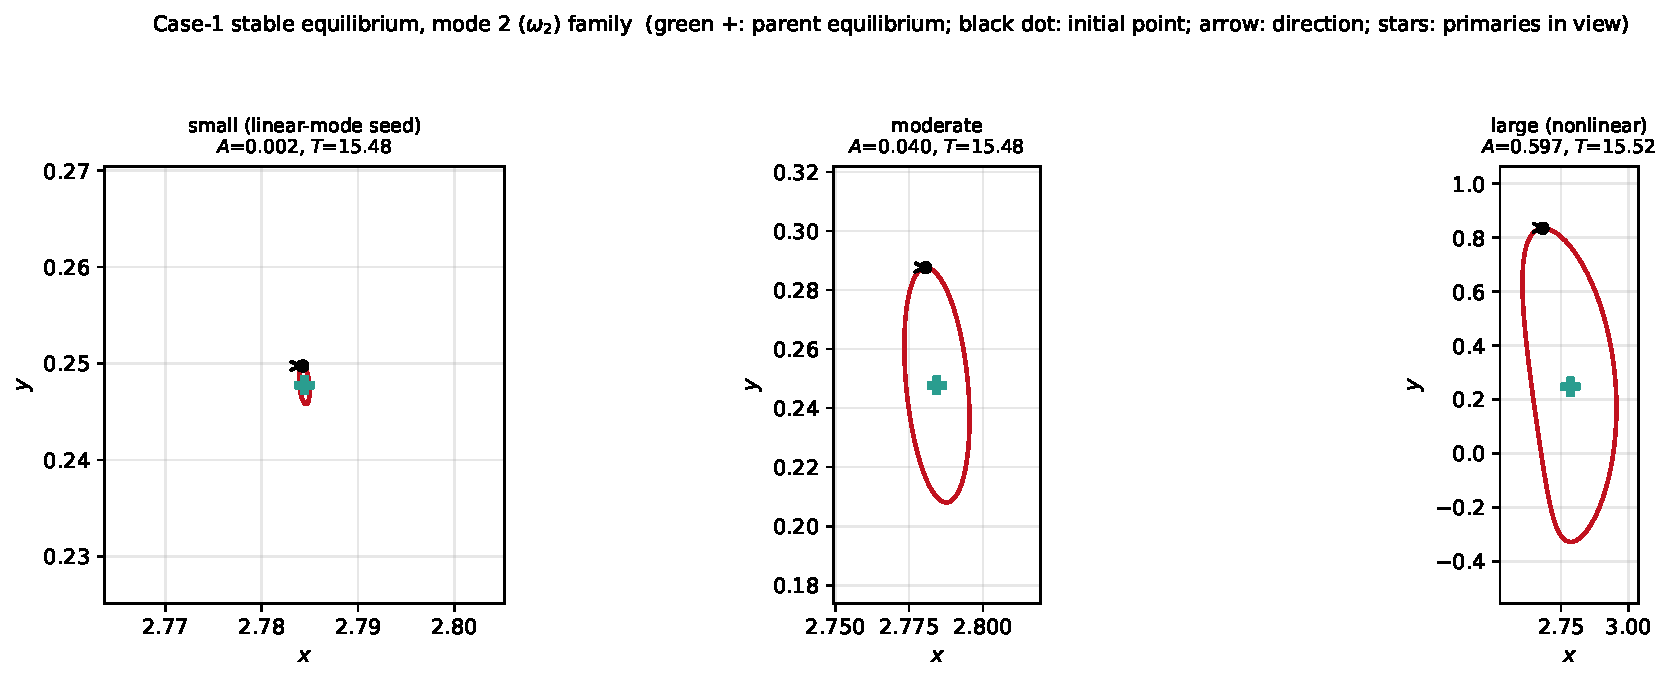
\includegraphics[width=\textwidth]{periodic_family_case1_mode2.pdf}
  \caption{Stable Lyapunov family from the Case-1 arc equilibrium (mode
  $\omega_2$): small (linear-mode seed), moderate, and large members. Green
  $+$: parent equilibrium; black dot: initial point; arrow: direction; stars:
  primaries in view. Floquet stable throughout.}
  \label{fig:family_case1}
\end{figure}
\begin{figure}[htbp]
  \centering
  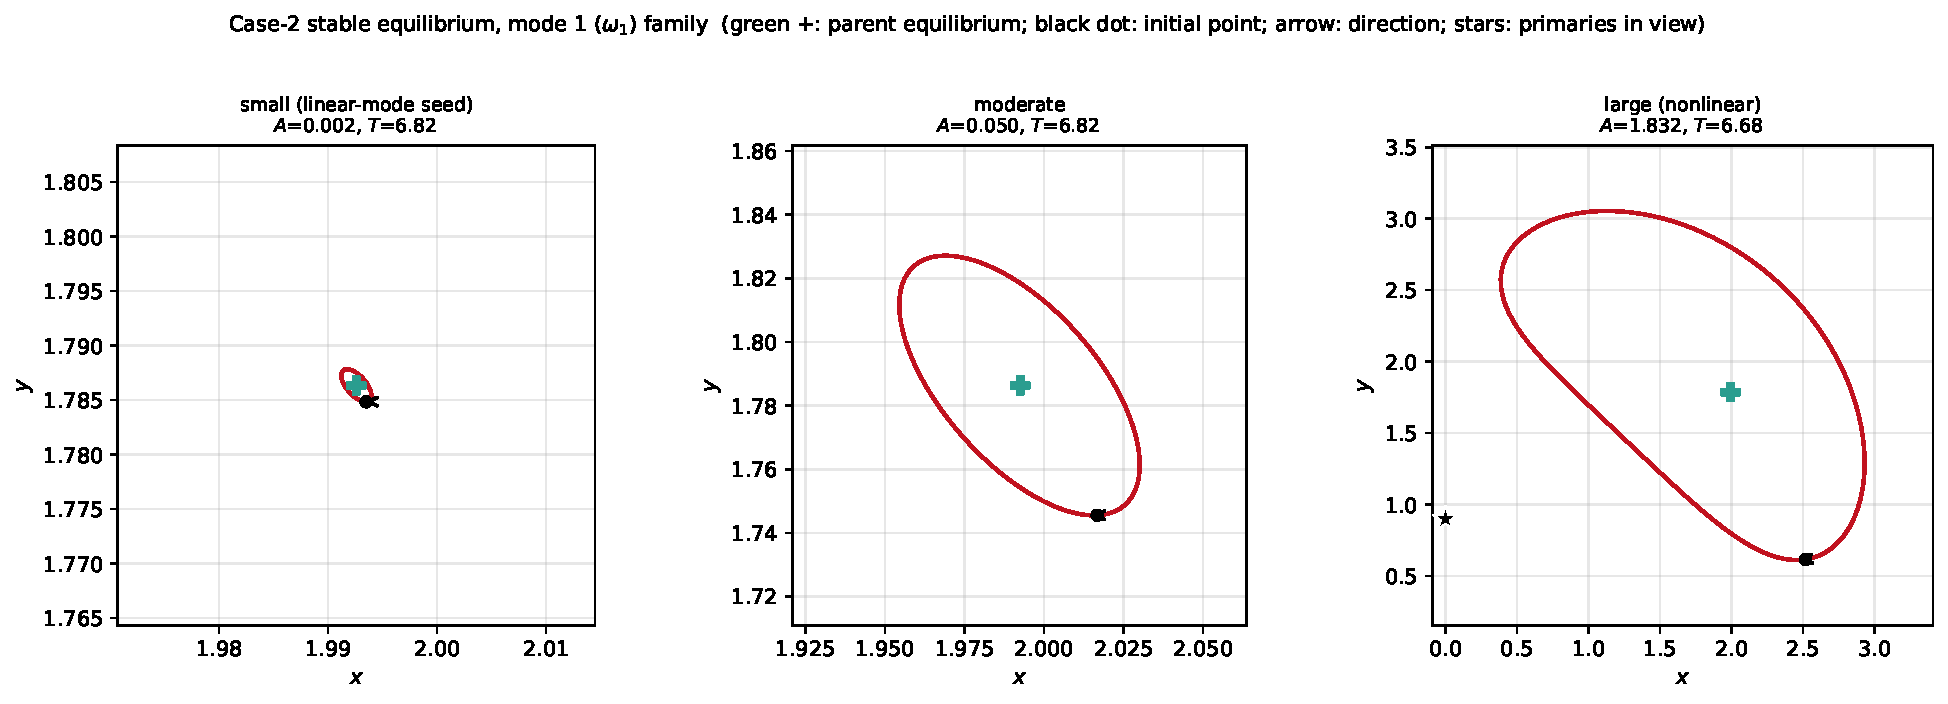
\includegraphics[width=\textwidth]{periodic_family_case2_mode1.pdf}
  \caption{Stable Lyapunov family from the Case-2 arc equilibrium (mode
  $\omega_1$). Floquet stable throughout.}
  \label{fig:family_case2}
\end{figure}
\begin{figure}[htbp]
  \centering
  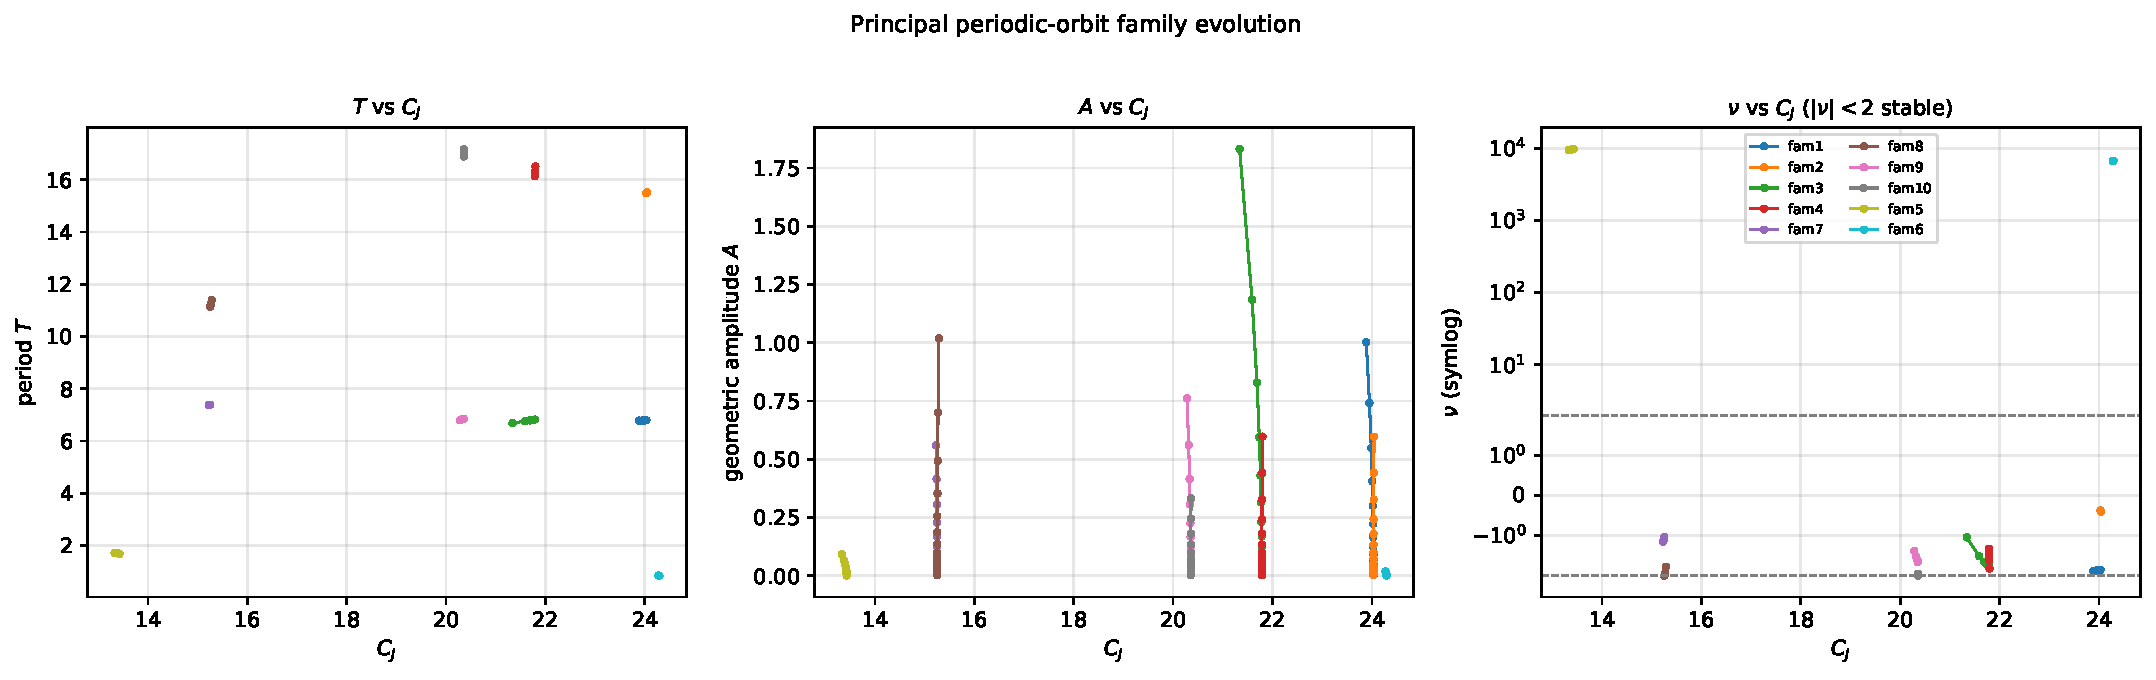
\includegraphics[width=\textwidth]{family_evolution.pdf}
  \caption{Family evolution: period $T$, geometric amplitude $A$, and Floquet
  index $\nu$ (symlog) against $C_J$. Real-unstable families (5, 6) sit at
  $\nu\sim10^{3}$; all others have $|\nu|<2$ over their computed range.}
  \label{fig:famevol}
\end{figure}
\begin{figure}[htbp]
  \centering
  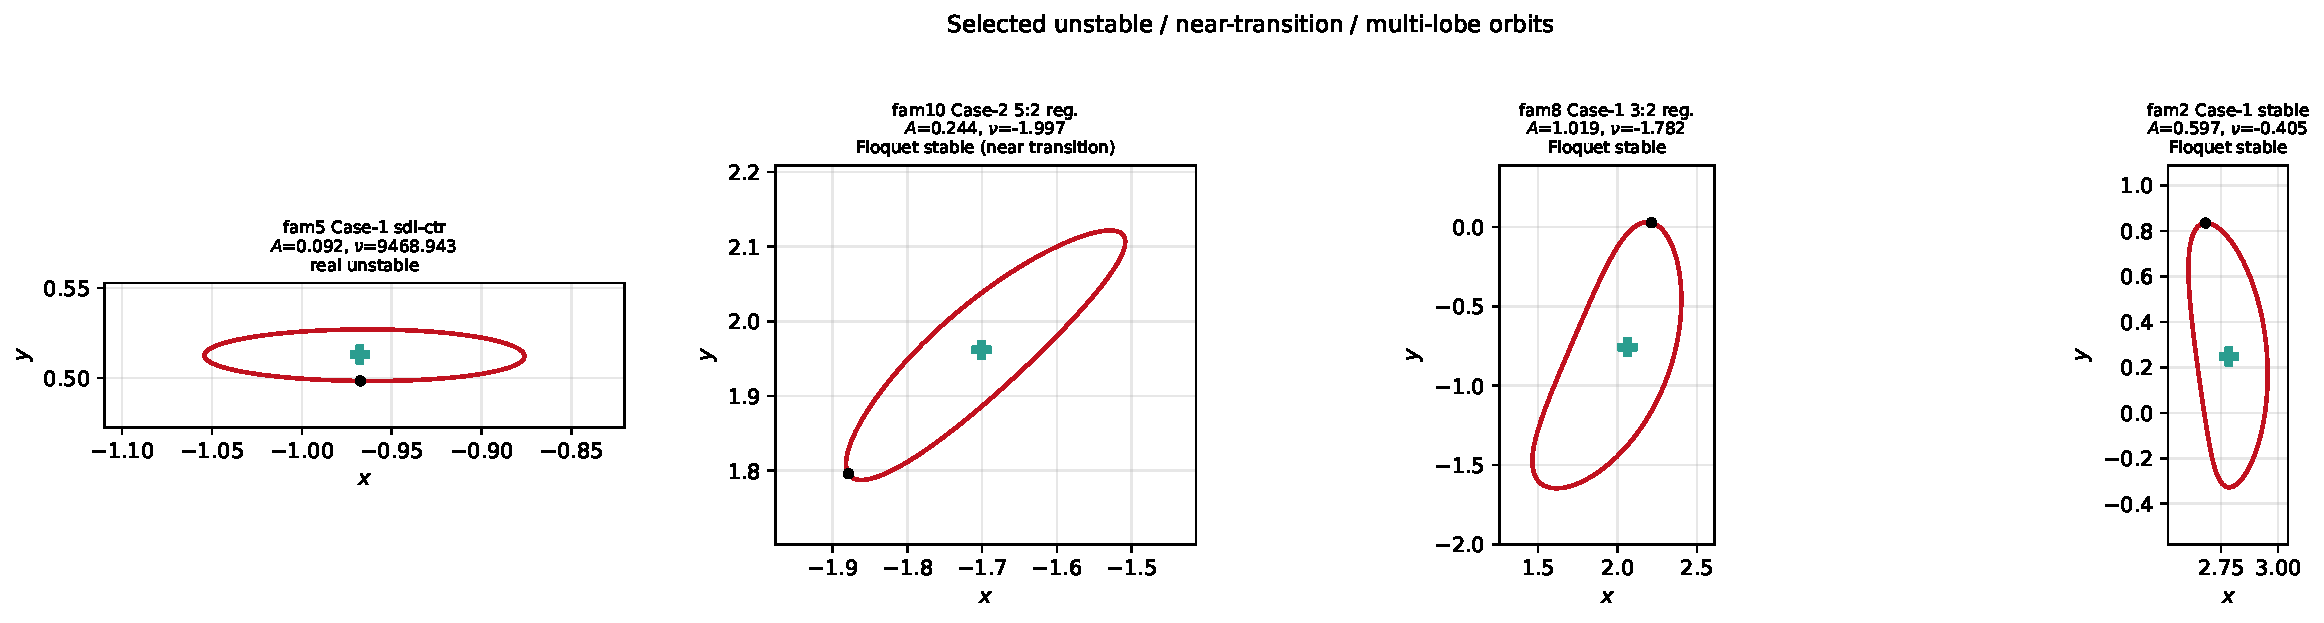
\includegraphics[width=\textwidth]{selected_resonant_orbits.pdf}
  \caption{Representative periodic orbits: a real-unstable orbit from a
  saddle$\times$centre parent (family~5), a near-period-doubling member of
  the Case-2 $5{:}2$ family (family~10), a multi-lobed member of the
  Case-1 $3{:}2$ family (family~8), and a large Floquet-stable orbit
  (family~2). Titles give the geometric amplitude, Floquet index $\nu$,
  and Floquet class.}
  \label{fig:selected_orbits}
\end{figure}
\begin{figure}[htbp]
  \centering
  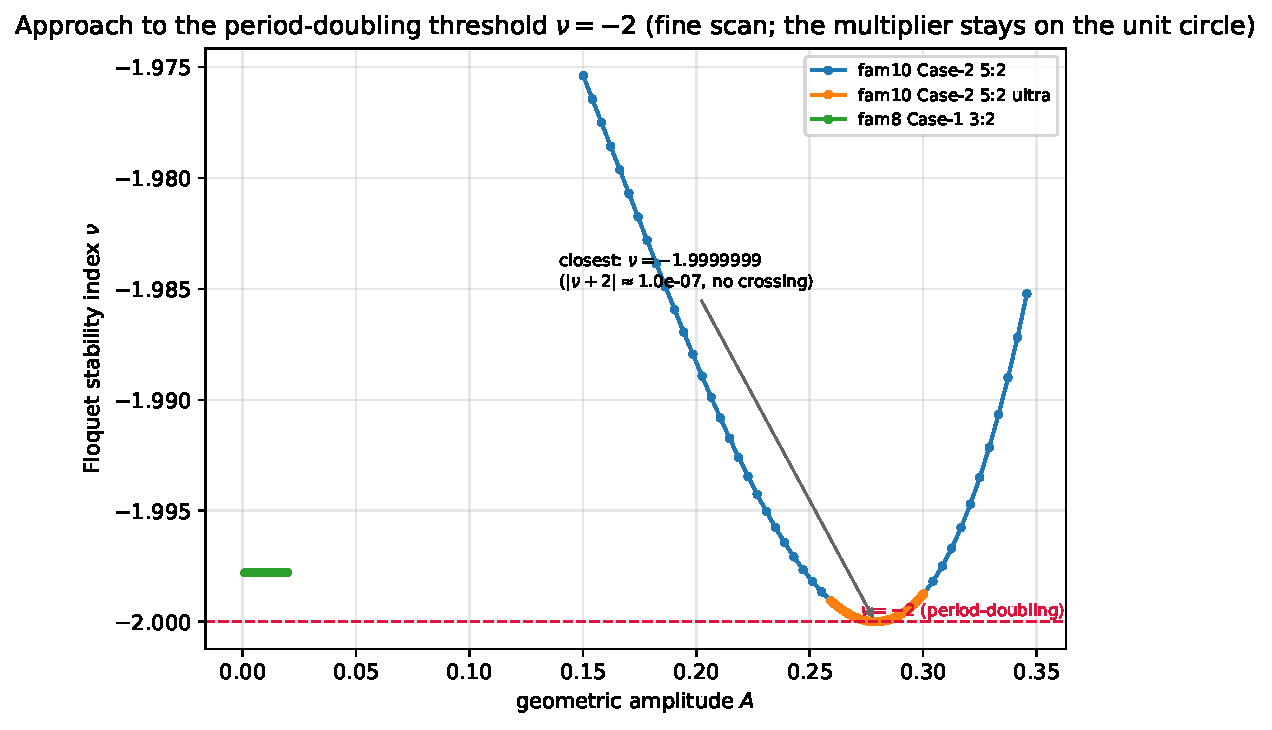
\includegraphics[width=0.72\textwidth]{period_doubling_scan.pdf}
  \caption{Fine scan of the Floquet index toward $\nu=-2$. Family~10 approaches
  the threshold to within $\sim10^{-7}$ and returns; the multiplier does not
  cross $-1$. No period-doubling bifurcation occurs.}
  \label{fig:period_doubling_scan}
\end{figure}

\section{Jacobi levels and Hill-region topology}
\label{sec:hill}

The Jacobi integral provides the geometric link between the equilibrium
bifurcations of Section~\ref{sec:results} and the periodic dynamics of
Section~\ref{sec:periodic}. We first follow the critical Jacobi values
associated with the equilibrium branches, then resolve one representative
change in Hill-region connectivity in the eleven-equilibrium regime, and
finally place selected periodic families within their corresponding
accessible regions.


\subsection{Critical Jacobi levels along the equilibrium branches}
\label{subsec:critical_jacobi}

Under the convention of Section~\ref{subsec:jacobi}, motion at Jacobi
constant $C_J$ is restricted to the Hill region
\begin{equation}
\mathcal H(C_J)
=
\left\{
(x,y):2\Omega(x,y)\geq C_J
\right\},
\label{eq:hill_region_results}
\end{equation}
whose boundary is the zero-velocity curve
\[
2\Omega(x,y)=C_J.
\]

Away from the primary singularities, the restricted equilibria are the
finite critical points of $\Omega$. Each equilibrium branch $L_i(s)$
therefore determines a critical Jacobi level
\begin{equation}
C_{J,i}(s)
=
2\Omega\!\left(L_i(s)\right).
\label{eq:critical_jacobi_branch}
\end{equation}
For a regular finite level set, changes in the topology of the Hill region
can occur only when $C_J$ passes through such a critical value. Depending
on the local type of the critical point, the change may involve the opening
or closing of a neck, the creation or loss of a bounded component, or a
change in the number of holes; a critical value does not therefore imply a
change in component count in every case.

Figure~\ref{fig:jacobi_levels} shows
$C_{J,i}(s)$ along the reliably tracked equilibrium branches. The
near-primary equilibria generally occupy the upper part of the critical
level ladder, whereas the more distant equilibria occur at lower levels.
Branches created or destroyed at the saddle-node folds introduce,
respectively remove, pairs of critical levels. At the fold itself the two
equilibrium branches coalesce at the same critical point and hence at the
same Jacobi value. The fold cascade of Section~\ref{sec:results} therefore
reorganizes not only the number of equilibria but also the hierarchy of
finite critical energy levels available to the restricted body.

\begin{figure}[htbp]
  \centering
  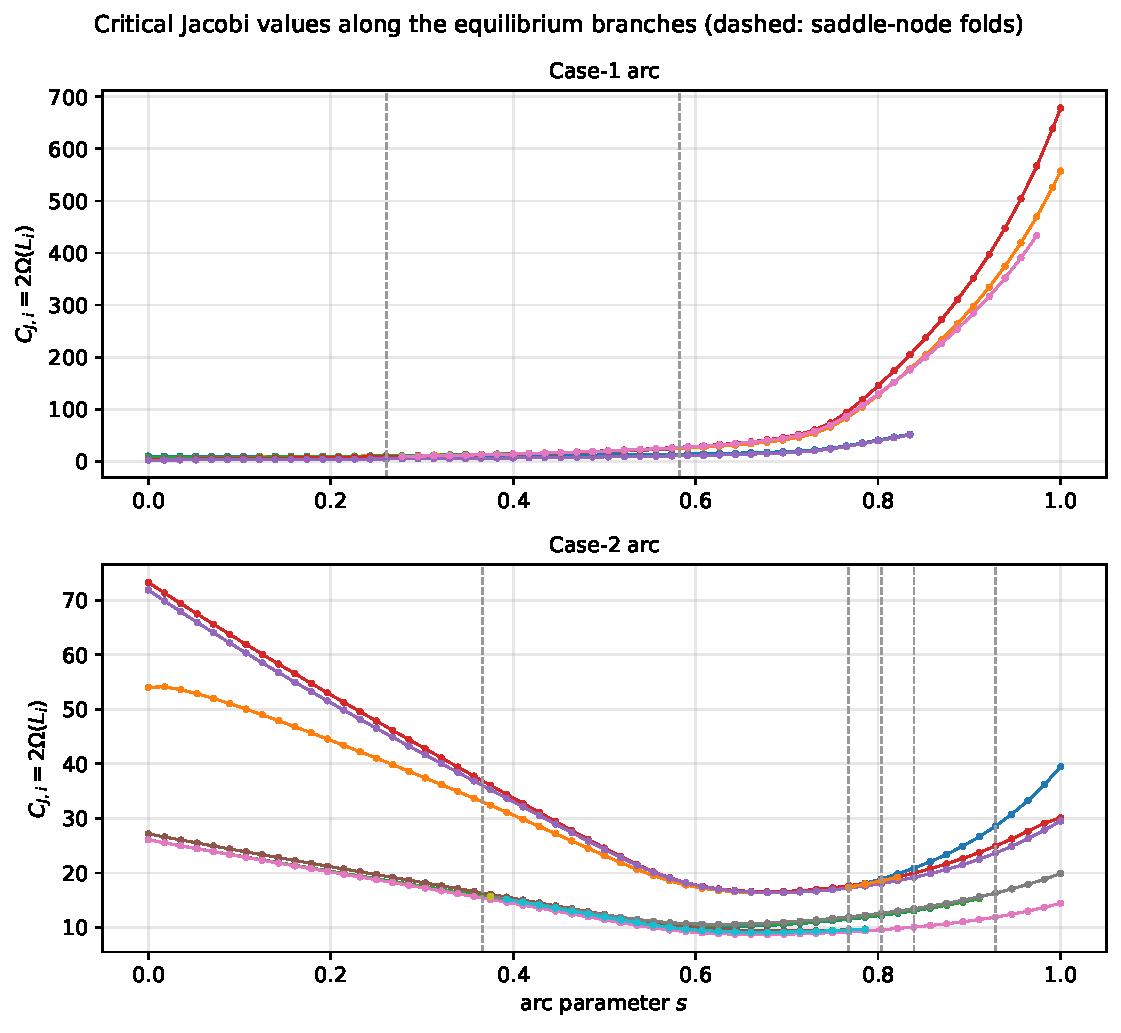
\includegraphics[width=\textwidth]{critical_jacobi_vs_s.pdf}
  \caption{Critical Jacobi values
  $C_{J,i}(s)=2\Omega(L_i(s))$ along the reliably tracked equilibrium
  branches of the two admissible arcs. Dashed vertical lines mark the
  saddle-node folds. Each curve gives a finite critical level at which the
  regular Hill-region topology may change.}
  \label{fig:jacobi_levels}
\end{figure}


\subsection{A representative connectivity change}
\label{subsec:hill_connectivity}

We resolve a representative connectivity change in the
eleven-equilibrium regime on the Case-2 arc, at
\[
s\simeq0.786,
\qquad
(c_1,c_2)\simeq(0.432,-0.602).
\]
Two Jacobi levels bracketing a portion of the interior critical-level
ladder are shown in the top row of Figure~\ref{fig:hill_regions}. They are
chosen as
\[
C_J=11.63
\qquad\text{and}\qquad
C_J=12.83,
\]
approximately $\pm0.6$ about the median equilibrium critical value
$C_J\simeq12.23$ at this configuration. The interval contains three finite
equilibrium critical values, approximately
\[
11.824,\qquad 11.924,\qquad 12.233.
\]

At $C_J=11.63$ the allowed set forms one connected component on the
computational domain, whereas at $C_J=12.83$ an inner allowed region has
detached from the outer region, giving two connected components. Increasing
$C_J$ across this interval therefore produces a net neck-closing transition
that separates a bounded inner component from the unbounded exterior
component. Because the interval spans a small cluster of critical values,
this calculation demonstrates the net connectivity change across that
portion of the critical-level ladder; it does not assign the transition to
one isolated critical equilibrium.

The component count is evaluated numerically by sampling
$2\Omega(x,y)$ on a uniform
\[
400\times400
\]
grid over
\[
[-6,6]^2,
\]
forming the binary allowed set
\[
2\Omega(x,y)\geq C_J,
\]
and applying four-connectivity labelling. Because
\[
2\Omega(x,y)\rightarrow+\infty
\]
both as a primary is approached and as
$\sqrt{x^2+y^2}\rightarrow\infty$, sufficiently small punctured
neighbourhoods of the primaries and the far exterior belong to the allowed
region for every finite $C_J$. No artificial exclusion mask is introduced
around the primaries in the component calculation.

The calculation was repeated on
\[
300\times300
\qquad\text{and}\qquad
500\times500
\]
grids. The detailed location and shape of the narrow neck are naturally
resolution dependent, but the reported change from one to two connected
components at the two quoted Jacobi levels is unchanged.

This calculation is intentionally representative rather than exhaustive.
Figure~\ref{fig:jacobi_levels} contains many other finite critical levels,
and crossing them need not always alter the component count; a complete
classification would require resolving the topology on both sides of every
critical level. We do not attempt that census here.


\subsection{Periodic families within the accessible regions}
\label{subsec:hill_orbits}

The lower panels of Figure~\ref{fig:hill_regions} place representative
Floquet-stable periodic orbits within the Hill regions corresponding to
their own Jacobi constants. The Case-2 example uses family~3 at
approximately
\[
C_J=21.34,
\]
while the Case-1 example uses family~2 at approximately
\[
C_J=24.04.
\]
In both cases the periodic orbit lies entirely inside a single connected
allowed region and remains separated from the zero-velocity boundary.

For the displayed trajectories we also evaluate the Hill margin
\[
\Delta_H(t)=2\Omega(x(t),y(t))-C_J.
\]
The minimum values along the plotted family-3 and family-2 members are
approximately
\[
0.529
\qquad\text{and}\qquad
2.65\times10^{-3},
\]
respectively. Both remain positive, confirming numerically that the
displayed trajectories remain inside the allowed region and do not
intersect the zero-velocity curve.

The examples illustrate the spatial distinction between the different
dynamical regimes encountered in Section~\ref{sec:periodic}. Periodic
librations associated with the selected outer doubly-elliptic equilibria
occupy broad allowed regions away from the most intricate near-primary
geometry, whereas periodic motion associated with inner
saddle$\times$centre equilibria occurs in a more strongly structured
near-primary region. The Hill geometry does not determine Floquet
stability, but it specifies the energetically accessible part of the plane
within which each periodic family must lie.

Taken together, Figures~\ref{fig:jacobi_levels} and
\ref{fig:hill_regions} illustrate the sequence
\[
\text{equilibrium bifurcation}
\longrightarrow
\text{critical Jacobi level}
\longrightarrow
\text{Hill-region topology}
\longrightarrow
\text{periodic dynamics}.
\]
The saddle-node cascade changes the set of finite critical values
$C_{J,i}(s)$; crossing those values can reorganize the accessible-region
topology; and the periodic families of Section~\ref{sec:periodic} are
confined to the resulting Hill regions. The present computation
demonstrates this connection through a resolution-checked representative
transition rather than a complete topological classification.

\begin{figure}[htbp]
  \centering
  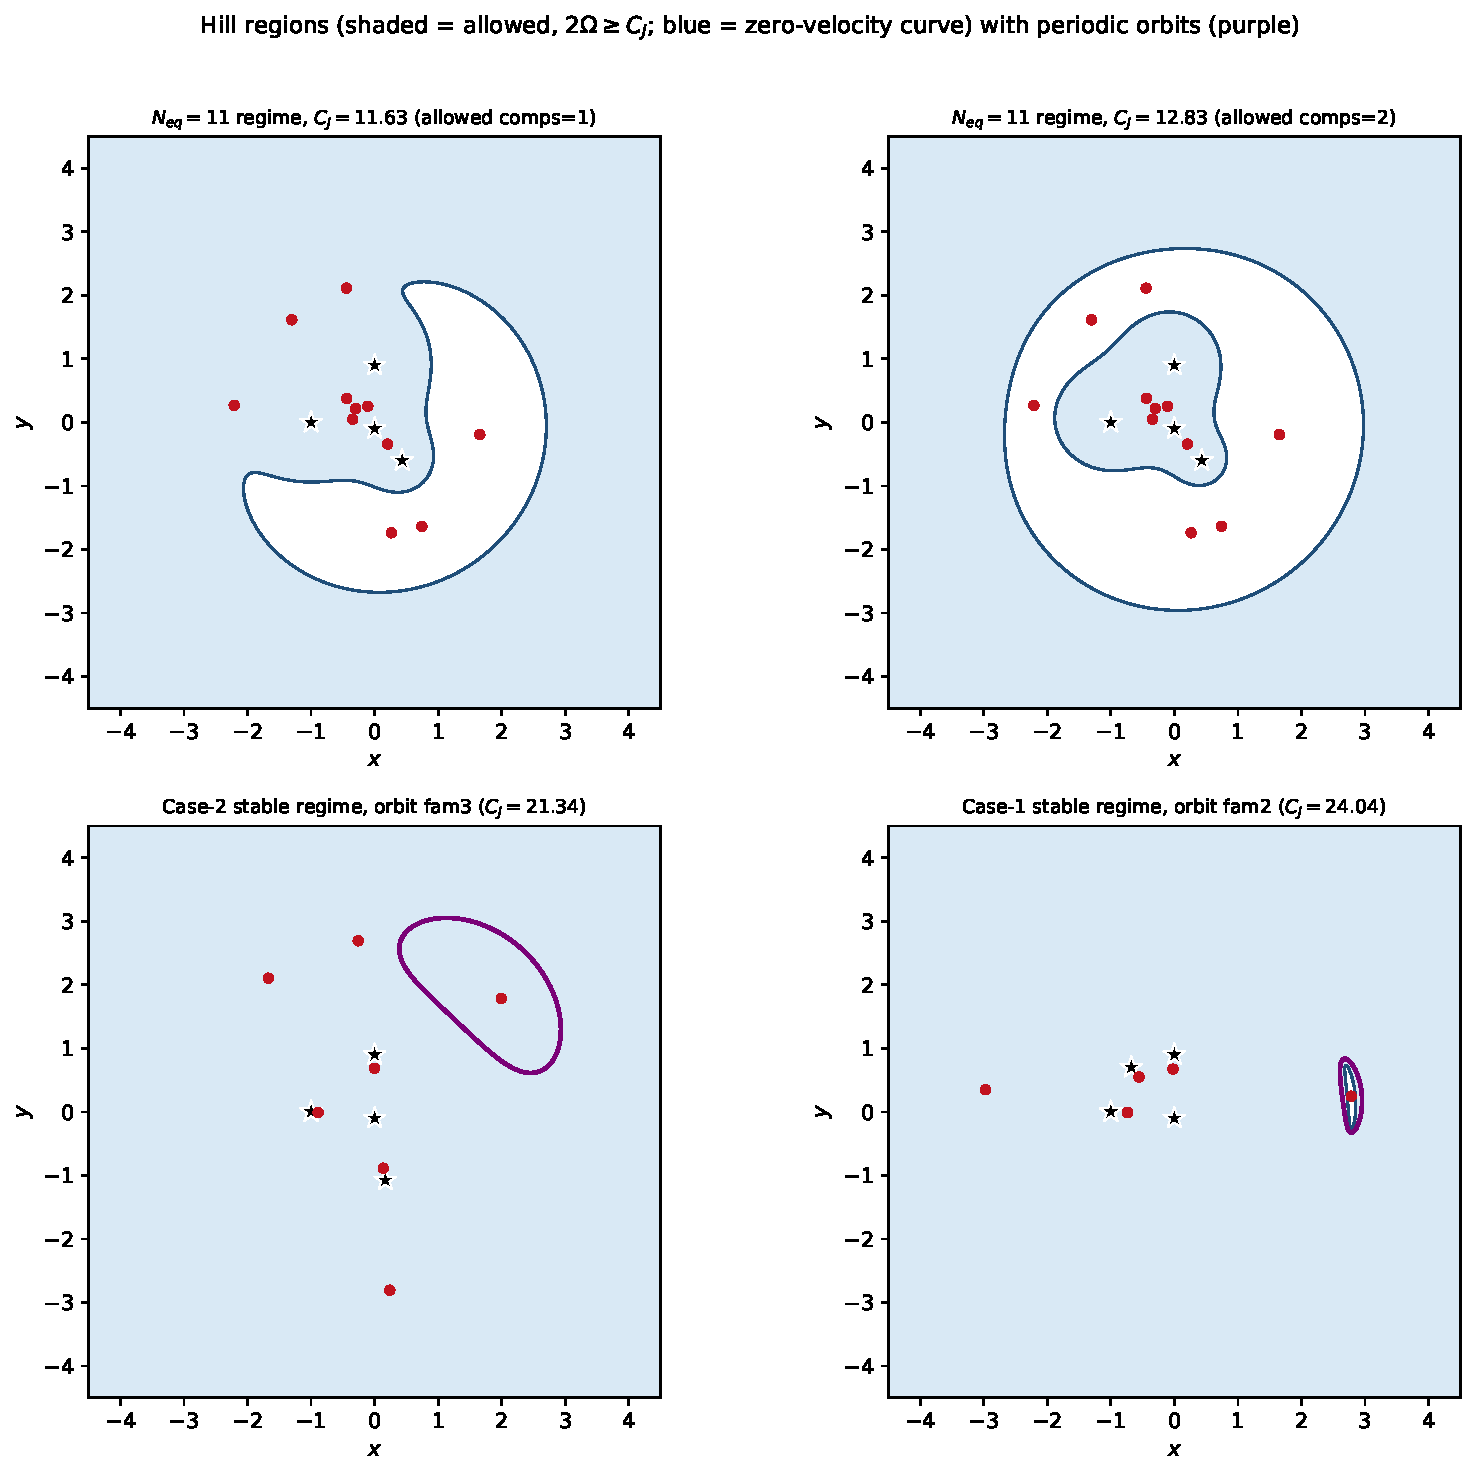
\includegraphics[width=0.95\textwidth]{hill_topology_with_orbits.pdf}
  \caption{Hill regions (shaded: allowed,
  $2\Omega\geq C_J$; blue: zero-velocity curve). Stars denote primaries,
  red points equilibria, and purple curves periodic orbits. Top: the
  eleven-equilibrium regime at $C_J=11.63$ (left) and $C_J=12.83$
  (right), bracketing a small cluster of finite critical Jacobi levels;
  the allowed set changes from one connected component to two across this
  interval as a neck closes.
  Bottom: representative Floquet-stable periodic orbits in the Case-2
  (family~3, left) and Case-1 (family~2, right) regimes, each shown at its
  own Jacobi constant.}
  \label{fig:hill_regions}
\end{figure}
\section{Discussion}
\label{sec:discussion}

The results reveal a hierarchy of structures linking the geometry of the
four-primary central configuration to the dynamics of the infinitesimal
body. The central-configuration set determines which primary geometries are
continuously accessible; along those components the restricted equilibria
undergo folds and changes of stability; the resulting centre modes generate
periodic-orbit families; and the associated critical Jacobi levels organize
the energetically accessible regions. We discuss these implications in
turn, together with the limits within which they have been established.


\subsection{Central-configuration topology and equilibrium bifurcation structure}
\label{subsec:discussion_cc}

The principal structural result is that equilibrium multiplicity cannot be
interpreted independently of the component structure of the underlying
central-configuration set. On the fixed slice
\[
(a,b)=(0.9,-0.1),
\]
the two reference configurations with five and nine restricted equilibria
belong to numerically distinct components of the regular zero set
$\psi=0$. Restricting these components to positive masses produces two
different admissible arcs. Consequently, the difference between the
five- and nine-equilibrium reference cases cannot be interpreted as the
result of a single bifurcation sequence connecting the two sampled
configurations.

This observation changes the role of the primary central configuration in
the restricted problem. Rather than serving only as a fixed background
geometry, its component structure determines which equilibrium branches
can coexist along a continuous deformation and which sequences of
bifurcations are accessible on that deformation. On the first admissible
arc the interior multiplicity sequence is
\[
5\rightarrow7\rightarrow5,
\]
before the positive-mass problem approaches a mass-vanishing boundary. On
the second arc the sequence is
\[
7\rightarrow9\rightarrow11\rightarrow9\rightarrow7\rightarrow5.
\]
Thus the equilibrium count is not a monotone measure of deformation or
asymmetry; it depends on the ordering of individual folds along the
admissible component.

The eleven-equilibrium interval illustrates why the scalar count alone is
an incomplete description. The pair $B_a$ created at the
$9\rightarrow11$ fold $F_4$ is not the pair destroyed at the subsequent
$11\rightarrow9$ fold $F_5$. Instead, the pre-existing pair $B_b$ is
destroyed at $F_5$, while $B_a$ persists until $F_6$. The two
nine-equilibrium intervals on either side of the eleven-equilibrium window
therefore have identical multiplicity but different branch populations.
A return to a previous value of $N_{\rm eq}$ does not imply a return to the
same equilibrium configuration.

The mechanisms responsible for changes of multiplicity must also be kept
distinct. The seven interior transitions are bifurcations of the restricted
equilibrium equations with all four primary masses positive. They satisfy
the numerical degeneracy and nondegeneracy conditions for generic
saddle-node folds and exhibit the expected square-root separation law.
By contrast, the Case-1 $5\rightarrow4$ transition occurs as
$\rho_2\rightarrow0$ near the boundary of the admissible primary set. It
is therefore a parameter-boundary degeneration of the four-primary problem
rather than an interior saddle-node bifurcation of the restricted dynamics.

These results suggest a broader organizing principle: in restricted
problems with sufficiently general primary geometries, the component
structure of the admissible primary-configuration set may organize the
accessible restricted bifurcation sequences. The present calculation
supports this interpretation on one two-dimensional slice only; whether it
persists in the full four-parameter admissible set or in other
non-symmetric restricted problems remains an open question.


\subsection{Stability and nonlinear periodic dynamics}
\label{subsec:discussion_dynamics}

The equilibrium continuation also shows that spectral stability is not
restricted to isolated symmetric configurations. Both admissible components
contain finite intervals on which selected libration points are
doubly elliptic. On the reliably tracked Case-1 branch this occurs over
approximately
\[
s\in[0.643,0.835],
\]
while the Case-2 component contains two distinct stable branches over
overlapping parameter ranges. In particular, two different spectrally
stable equilibria coexist near
\[
s\simeq0.196,
\]
one close to a $5{:}2$ centre-frequency commensurability and the other
close to $2{:}1$. This coexistence reinforces the conclusion that neither
the arc coordinate $s$ nor the equilibrium count by itself uniquely
characterizes the local dynamics; equilibrium branch identity is also
required.

The centre modes of the selected equilibria organize the local nonlinear
periodic dynamics. At each parent used in Section~\ref{sec:periodic}, the
selected imaginary eigenvalue satisfies the exact non-resonance condition
required by the Lyapunov centre theorem. The ten computed families are
therefore Lyapunov families in the local theorem sense, including those
continued from saddle$\times$centre parents. What differs is their
stability.

For the selected doubly-elliptic parents, the computed families retain
their nontrivial Floquet multipliers on the unit circle throughout the
continued intervals and are therefore Floquet stable in the sense defined
in Section~\ref{subsec:floquet}. This is a periodic-orbit statement and
should not be interpreted as a proof of nonlinear or KAM stability.
Conversely, families~5--6 originate from saddle$\times$centre parents.
Their centre directions still generate valid Lyapunov families, but the
continued periodic orbits possess a strongly real reciprocal Floquet pair
and are correspondingly real unstable. The existence of a local periodic
family and its Floquet stability are therefore logically distinct
questions.

The low-order centre-frequency near-commensurabilities provide useful
locations at which to examine possible changes in periodic-orbit stability,
but they must not be confused with exact resonances. Families~7--8 are
continued from the Case-1 parent near $3{:}2$, while families~9--10 use the
distinct Case-2 parent near $5{:}2$. In both cases the parent frequency
ratio differs from the exact rational value, so the Lyapunov-centre
non-resonance condition remains satisfied.

The most pronounced nonlinear stability feature occurs on family~10. Its
nontrivial Floquet pair approaches the period-doubling collision at
\[
\nu=-2
\]
to within approximately
\[
|\nu+2|\simeq10^{-7}.
\]
An ultra-fine amplitude sweep with step $8\times10^{-4}$ resolves the
minimum and shows the index turning back without crossing the threshold.
The computed family therefore provides no evidence of a period-doubling
bifurcation over the continuation interval investigated. Family~8 also
approaches the same boundary, but only to within approximately
$2\times10^{-3}$.

This negative result should be interpreted narrowly. The multiplier scans
show no crossing of the selected low-order conditions
\[
\nu=2,\qquad
\nu=0,\qquad
\nu=-1,\qquad
\nu=-2
\]
along the computed portions of the ten families. We have not performed an
independent exhaustive search for all secondary periodic families, nor
does the absence of a crossing on these continuation intervals exclude
period-doubled or resonant solutions elsewhere in parameter or phase space.

The Jacobi and Hill-region calculations provide the geometric context for
these periodic motions. The equilibrium branches determine a ladder of
critical Jacobi values, and changes across these levels can reorganize the
accessible region. The representative Case-2 calculation demonstrates a
net change from one to two connected Hill components across a cluster of
three nearby critical levels. The periodic examples then show selected
Floquet-stable families embedded within the allowed regions at their own
Jacobi constants. The Hill geometry determines where motion at a given
energy is possible, but it does not determine the Floquet stability of the
orbit contained within that region.


\subsection{Relation to previous models, scope and limitations}
\label{subsec:discussion_scope}

The present problem differs structurally from the symmetric restricted
five-body models most commonly treated in the literature. In those models,
reflection, permutation, or rotational symmetry constrains the primary
geometry to a prescribed low-dimensional family. For example, Ollongren's
symmetric restricted five-body configuration supports nine libration
points, including stable equilibria \cite{ollongren1988}, while the ring
problem and other symmetric formulations exploit rotational or reflection
structure to organize their equilibrium and periodic-orbit families
\cite{kalvouridis1999,zotospapadakis2019,zotossuraj2018}. Symmetric
four-body central configurations such as the Caledonian and kite families
similarly restrict the primary configuration to a special geometric locus
\cite{stevesroy1998,benhammouda2020}.

The distinction in the present problem is not merely that the equilibrium
count is larger. On the investigated non-symmetric slice, the admissible
central-configuration set itself separates into different components, and
the restricted equilibrium multiplicity must therefore be interpreted
component by component. The eleven-equilibrium state exceeds the
nine-equilibrium counts reported in the symmetric restricted five-body
examples cited above, but its more significant feature is that it arises
within a continuously resolved saddle-node cascade and contains a branch
exchange. Likewise, the periodic families are continued from
asymmetrically located equilibria using a general shooting formulation and
full-monodromy Floquet analysis rather than being constructed through an
assumed reflection symmetry. The comparison with previous work is therefore
primarily structural rather than a quantitative comparison at matched
masses.

Several limitations delimit these conclusions. First, all primary
continuation is carried out on the fixed slice
\[
(a,b)=(0.9,-0.1).
\]
The numerically distinct components identified there need not remain
disconnected when $a$ and $b$ are allowed to vary. Determining the topology
of the complete admissible set would require continuation in the full
four-dimensional geometric parameter space.

Second, equilibrium completeness is numerical rather than analytic. The
reported multiplicities are supported by deterministic grid searches,
fixed-seed random starts, local searches around the primaries, strict
residual tests, and an expanded re-search of the eleven-equilibrium
configuration. These procedures provide strong numerical evidence for the
reported counts under the stated search protocol, but they do not provide
an analytic upper bound on the number of real equilibria.

Third, branch tracking becomes unreliable near the mass-vanishing limits
where some equilibria recede rapidly. Such points are explicitly flagged
and excluded from branch-dependent stability, centre-frequency, Jacobi,
and periodic-orbit claims. The reliably tracked intervals are therefore
shorter than the full ranges over which individual numerical roots may
still be found.

Fourth, the periodic-orbit calculations use natural amplitude continuation
rather than pseudo-arclength continuation. The reported 198 solutions
therefore represent the portions of ten families accessible while the
chosen amplitude remains a useful continuation coordinate; they are not
claimed to be maximal families. Likewise, no systematic continuation of
secondary resonant or period-doubled branches has been undertaken.

Fifth, the Hill-region calculation is representative rather than
exhaustive. The connectivity change reported in Section~\ref{sec:hill} is
resolution-checked on $300^2$, $400^2$, and $500^2$ grids, but the selected
Jacobi interval spans three nearby equilibrium critical values. The
calculation therefore establishes a net $1\rightarrow2$ connectivity
change across that part of the critical-level ladder rather than assigning
the change to one particular critical equilibrium. A complete topological
classification would require resolving the Hill geometry on both sides of
every relevant critical level.

Finally, the stability results have deliberately limited meaning. We
establish spectral stability of equilibria and Floquet stability of
periodic orbits. We do not establish nonlinear, orbital, or KAM stability,
and finite-time numerical boundedness is not used as a substitute for any
of these notions.

Within these limits, the principal structural conclusions are robust: on
the investigated slice the admissible central-configuration component
structure organizes the accessible equilibrium bifurcation sequences;
those sequences contain generic folds, stable-equilibrium intervals, and a
branch-exchange eleven-equilibrium regime; and selected centre modes extend
to well-resolved Lyapunov periodic families whose Floquet behaviour and
Hill-region setting can be followed quantitatively.
\section{Conclusions and outlook}
\label{sec:conclusions}

We have studied how the equilibrium structure, linear stability, and local
periodic dynamics of an infinitesimal fifth body change as a general
non-symmetric four-primary central configuration is continuously deformed.
Rather than comparing isolated primary configurations, the analysis follows
the admissible central-configuration set itself and resolves the restricted
equilibria, their bifurcations, and selected periodic-orbit families along
that set.

Three conclusions emerge.

First, on the investigated slice
\[
(a,b)=(0.9,-0.1),
\]
the admissible central-configuration set is numerically separated into two
distinct components containing the Case-1 and Case-2 reference
configurations. The five- and nine-equilibrium cases therefore do not lie
on a single fixed-$(a,b)$ continuation family. This establishes that
equilibrium multiplicity must be interpreted together with the component
structure of the underlying primary configuration: different sampled
counts need not be connected by a bifurcation sequence on the same
admissible component. The result is specific to the investigated slice and
does not establish disconnection in the full four-parameter admissible set.

Second, the restricted equilibrium structure along these components is
organized by seven generic saddle-node folds. The corresponding interior
multiplicity sequences are
\[
5\rightarrow7\rightarrow5
\]
on the Case-1 component and
\[
7\rightarrow9\rightarrow11\rightarrow9\rightarrow7\rightarrow5
\]
on the Case-2 component. The Case-1 arc additionally exhibits a
mass-vanishing boundary degeneration as $\rho_2\rightarrow0$, which is
distinct from the interior folds. The eleven-equilibrium interval is
structurally significant because it contains a branch exchange: the pair
$B_a$ created at the $9\rightarrow11$ fold is not the pair $B_b$
destroyed at the following $11\rightarrow9$ fold. Thus two configurations
can have the same equilibrium count while containing different sets of
equilibrium branches. The scalar multiplicity is therefore only a coarse
description of the underlying equilibrium structure.

Third, this equilibrium organization is inherited by the local dynamics.
Both admissible components contain reliably resolved intervals of
spectrally stable equilibria, and the Case-2 component supports two
distinct spectrally stable equilibrium branches over overlapping parameter
ranges. From selected simple centre modes we computed ten Lyapunov
periodic-orbit families comprising 198 corrected solutions. The families
continued from the selected doubly-elliptic parents remain Floquet stable
over the computed intervals, whereas the families continued from selected
saddle$\times$centre parents possess a real reciprocal Floquet pair and are
real unstable.

Low-order centre-frequency ratios encountered along the stable branches are
near-commensurabilities rather than exact resonances at the parent
equilibria. Families~7--8 sample the Case-1 region near $3{:}2$, while
families~9--10 sample the distinct Case-2 region near $5{:}2$. Family~10
approaches the period-doubling boundary extremely closely,
\[
\min |\nu+2|\simeq10^{-7},
\]
but an ultra-fine amplitude sweep resolves a turn-back rather than a
crossing. No period-doubling bifurcation is therefore detected on the
computed portion of that family. More generally, no crossing of the
selected low-order multiplier conditions is found along the ten continued
families; this does not exclude secondary periodic solutions elsewhere in
parameter or phase space.

The equilibrium structure also determines a hierarchy of critical Jacobi
levels. A representative calculation in the eleven-equilibrium regime
shows a resolution-robust net change in Hill-region connectivity from one
component to two across a small cluster of three nearby equilibrium
critical levels. Representative Floquet-stable periodic orbits remain
inside the corresponding allowed regions at their own Jacobi constants.
This provides a concrete geometric link between the equilibrium
bifurcations, the critical energy levels, the accessible Hill geometry, and
the periodic dynamics without implying that every critical level produces
a change in component count.

Taken together, the results support a broader interpretation: in a
non-symmetric restricted problem, the topology of the admissible
primary-configuration set can itself act as an organizing structure for the
restricted dynamics. On the present slice it determines which equilibrium
branches can coexist and which bifurcation sequences are accessible; those
branches in turn determine the available centre modes, critical Jacobi
levels, and local periodic families. Whether this organizing role persists
in the full parameter space is a natural question for further study.

Several extensions follow directly from the present analysis. The most
important is continuation in the complete four-parameter admissible
central-configuration set, which would determine whether the two components
identified here remain disconnected when $a$ and $b$ are also allowed to
vary. A second direction is pseudo-arclength continuation of the
periodic-orbit families themselves, together with targeted continuation of
secondary branches near the observed low-order commensurabilities and the
near-period-doubling point. A third is a systematic Hill-region
classification across individual critical Jacobi levels rather than the
representative connectivity calculation performed here. Finally, comparison
with symmetric restricted five-body models at matched or otherwise
controlled mass configurations would help separate effects caused by mass
distribution from those caused specifically by the geometry and topology
of the admissible central-configuration set.


\section*{Data and code availability}
The model, continuation, bifurcation, stability, and periodic-orbit
computations, together with the scripts that generate every table and figure in
this paper deterministically from the verified result files, are organized as a
single release archive. Every numerical result was produced with
\emph{Python~3.14.5} and \emph{NumPy~2.5.0}, \emph{SciPy~1.17.1},
\emph{Matplotlib~3.10.9}, and \emph{pandas~3.0.3}; integrations use
\texttt{scipy.integrate.solve\_ivp} with the \texttt{DOP853} method at
$\mathrm{rtol}=\mathrm{atol}=10^{-12}$, and all random seeds are fixed, so the
pipeline is designed to be deterministically reproducible within the pinned
software environment. The exact code and result set will be deposited in a public
repository and a permanent archive \emph{at submission}, and the following
identifiers completed: \emph{repository:} [URL];\ \emph{commit/tag:} [hash];\
\emph{archive DOI:} [DOI]. Full numerical settings and per-file provenance are
documented in the accompanying reproducibility protocol.

\bibliographystyle{plain}
\bibliography{references}

\end{document}
